\documentclass[11pt]{scrartcl}
 
%deutsche Zeichensätze einbinden
\usepackage{ucs}
\usepackage[utf8x]{inputenc}
\usepackage[T1]{fontenc}

%Latex mitteilen, dass deutsche sprache verewendet wird
\usepackage[ngerman]{babel}

%Mathepackage der American Mathematical Society einbinden 
\usepackage{amsmath,amssymb,amstext}

%Graphic package einbinden
\usepackage{graphicx}
\usepackage{subfigure} 

\usepackage{listings} 
\usepackage{xcolor}

%Autor,... festlegen
\title{Embedded Systems 1 - Dokumentation}
\author{Kevin Fritz}
\date{\today{}, Aalen}

% für Listings
\usepackage{listings}
\lstset{numbers=left, numberstyle=\tiny, numbersep=5pt, keywordstyle=\color{blue}\bfseries, stringstyle=\ttfamily,showstringspaces=false,basicstyle=\footnotesize,captionpos=b,tabsize=2,}

%define language and add more keywords
%\lstset{language=C, %morekeywords={[2]uint8_t,uint16_t,uint32_t,uint64_t,int8_t,int16_t,int32_t,int64_t,__asm__},
%morekeywords={[3]TRISB8,ANSB8,CNIENB8,CNPUB8,CNPB8}
%}

\definecolor{bluekeywords}{rgb}{0,0,1}
\definecolor{greencomments}{rgb}{0,0.5,0}
\definecolor{redstrings}{rgb}{0.64,0.08,0.08}
\definecolor{xmlcomments}{rgb}{0.5,0.5,0.5}
\definecolor{orangestrings}{rgb}{1,0.5,0}
\definecolor{bluetypes}{rgb}{0,0.7,1}
\definecolor{types}{rgb}{0.17,0.57,0.68}

\lstset{language=C,
captionpos=b,
%numbers=left, %Nummerierung
%numberstyle=\tiny, % kleine Zeilennummern
frame=lines, % Oberhalb und unterhalb des Listings ist eine Linie
showspaces=false,
showtabs=false,
breaklines=true,
showstringspaces=false,
breakatwhitespace=true,
escapeinside={(*@}{@*)},
commentstyle=\color{xmlcomments},
morekeywords={__asm__},
morekeywords=[2]{uint8_t,uint16_t,uint32_t,uint64_t,int8_t,int16_t,int32_t,int64_t,STATE_STABLE_HIGH, STATE_INSTABLE_HIGH, STATE_STABLE_LOW, STATE_INSTABLE_LOW, LOW, HIGH},
morekeywords={[3]TRISB8,ANSB8,CNIEB8,CNPUB8,CNPDB8, LATB8},
keywordstyle=\color{bluekeywords},
keywordstyle=[2]\color{bluetypes},
keywordstyle=[3]\color{greencomments},
stringstyle=\color{orangestrings},
basicstyle=\ttfamily\small,
}



\usepackage[
colorlinks=true,
urlcolor=blue,
linkcolor=black
]{hyperref}

\begin{document}
%Titelblatt einfügen
\maketitle
\begin{center}
	
\includegraphics[width=\textwidth]{Images/hs_aalen_logo}
\end{center}
\newpage

\tableofcontents
\newpage

\addsec{Einleitung} %addsec erhält keine nummerrierung
\label{sec:einleitung} %label erstellen für quervereise
Einleitung muss noch verfasst werden.
\newpage

\section{Getting Started}
\subsection{Aufgabenstellung}

\begin{enumerate}%Aufzählung mit Numerierung
		\item Nehmen Sie das Programm „HelloWorld2“ in Betrieb.
		\item Entfernen Sie die Verzögerungsfunktion und messen Sie die Frequenz, mit der die LED angesteuert wird. Überprüfen Sie das Ergebnis durch Analyse des generierten Assembler-Codes. Wie groß ist die Rechenleistung in MIPS?
		
		\item Erhöhen Sie die CPU-Frequenz auf den maximal möglichen Wert. Weisen Sie durch eine Messung nach, dass die CPU-Frequenz tatsächlich erhöht wurde. Wie groß ist die Rechenleistung in MIPS?
\end{enumerate}


\subsection{Lösung}
\begin{enumerate}
		\item Programm „HelloWorld2“ in Betrieb nehmen. Der Programmcode ist in Listing \ref{lst:HelloWorld2} zu sehen.
		\item Die Verzögerungsfunktion wurde auskommentiert. Der Oszi-Aufnahme aus Abbildung \ref{image:AnsteuerungsfrequenzLED} kann entnommen werden, dass die Zeitdauer um einen Port ein- bzw. auszuschalten jeweils ungefähr $5,75us$ beträgt. Daraus ergibt sich eine Frequenz von $f=\frac{1}{T}=\frac{1}{5,75us}≈174kHz$. Aus Listing \ref{lst:AssemblerToggle} geht hervor das zum Toggeln der LED 16 Assemblerbefehle benötigt werden.
		\begin{equation}
		\label{eq:MIPS}
		MIPS=\frac{16}{5,75us}*10^{-6}≈2,783  MIPS
		\end{equation}
		Die Einheit MIPS gibt an, wie viele Maschinenbefehle (Instruktionen) ein Mikroprozessor pro Sekunde ausführen kann. 1 MIPS bedeutet, er kann eine Million Maschinenbefehle pro Sekunde ausführen. MIPS ist eine ungenaue Einheit, da verschiedene Assemblerbefehle verschieden viel Zeit benötigen.
		\item Um die CPU-Frequenz auf den Maximalen Wert zu erhöhen wird die auf dem Board verbaute PLL verwendet. Die Parameter zur Konfiguration der PLL sind dem Datenblatt (Abbildung \ref{image:CPUClockingSystem}) zu entnehmen. Der Wertebereich der PLL Parameter kann Abbildung \ref{image:PLLParameter} entnommen werden. Die Parameter wurden (mit einem Excel Sheet, Abbildung \ref{image:PLLParameterExcel}) so ausgelegt, dass sich eine Taktfrequenz $F_{OSC}$ von $140 MHz$ ergibt. Aus dem Oszillator Modul (online zu finden bei mikrochip) kann eine Code-Sequenz entnommen werden wie die jeweiligen PLL-Parameter zu setzen sind. Der Ausschnitt aus dem Datenblatt wurde für unsere Zwecke angepasst (Listing \ref{lst:OscillatorSetup}).\newline		
		Nach Konfigurieren der PLL wurde wieder die Zeitdauer zum toggeln der LED gemessen ($302ns$ für 16 Assembler-Befehle), hieraus ergibt sich eine Rechenleistung von:
		\begin{equation}
		\label{eq:MIPS_140MHz}
		MIPS=\frac{16}{302ns}*10^{-6}≈52,980  MIPS
		\end{equation}
		Setzt man die ausgerechneten MIPS ins Verhältnis, kommt man zu dem Entschluss das die gemessenen Werte plausibel sind, da: $2,783*\frac{140}{7,37}≈52,867 $.
		
		
\end{enumerate}

\newpage
%\lstset{language=C}
\begin{lstlisting}[frame=htrbl, caption={Quellcode HelloWorld2}, label={lst:HelloWorld2}]
// Check for Project Settings
#ifndef __dsPIC33EP512MU810__
#error "Wrong Controller"
#endif
#include <xc.h>    //Include appropriate controller specific headers
#include <stdint.h>//Standard typedefs
// Oscillator Configuration
_FOSCSEL(FNOSC_FRC); //Initial Oscillator:  Internal Fast RC
_FOSC(POSCMD_NONE);  //Primary Oscillator disabled (not used)

/* Substitute for stdlib.h */
#define	EXIT_SUCCESS	0
#define	EXIT_FAILURE	1

/* Hardware  */
#define _LED200 LATBbits.LATB8

void delay_ms(uint16_t u16milliseconds){
	uint16_t ui16_i=0;
	while(u16milliseconds){
		for (ui16_i=0;ui16_i<331;ui16_i++){//1 ms delay
			__asm__ volatile("nop \n\t"
			"nop \n\t"
			"nop \n\t");
		}//for
	u16milliseconds--;
	}//while
}
int main() {
/* Port Configurations */ // DS70616G-page 209
// ODCB (open drain config) unimplemented (DS70616G, Table 4-56)
ANSELBbits.ANSB8=0;     //Digital I/O
CNENBbits.CNIEB8=0;     //Disable change notification interrupt
CNPUBbits.CNPUB8=0;     //Disable weak pullup
CNPDBbits.CNPDB8=0;     //Disable weak pulldown
TRISBbits.TRISB8=0;     //Pin B8: Digital Output
LATBbits.LATB8=0;       //Pin B8: Low
/* Endless Loop */
while(1){
	/* LATBbits.LATB8 = !(LATBbits.LATB8); //Toggle Pin B8 */
	_LED200=!_LED200; //Toggle LED
	delay_ms(500);
}//while
return (EXIT_SUCCESS);  //never reached
} //main()
\end{lstlisting}
\newpage
\begin{figure}
	\centering
	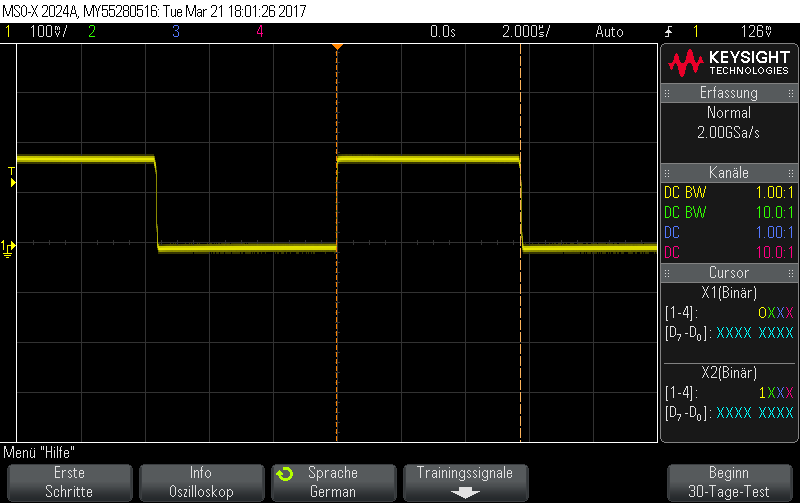
\includegraphics[width=\textwidth]{Images/1_1_MIPS}
	\caption[AnsteuerungsfrequenzLED]{Ansteuerungsfrequenz der LED}
	\label{image:AnsteuerungsfrequenzLED}
\end{figure}


\begin{lstlisting}[frame=htrbl, caption={Assembler Befehle zum toggeln}, label={lst:AssemblerToggle}]
//while(1){
// _LED200=!_LED200; //Toggle LED
00033E  8070A1     MOV LATB, W1
000340  201000     MOV #0x100, W0
000342  608000     AND W1, W0, W0
000344  A7F000     BTSC W0, #15
000346  EA0000     NEG W0, W0
000348  E90000     DEC W0, W0
00034A  DE004F     LSR W0, #15, W0
00034C  784000     MOV.B W0, W0
00034E  FB8000     ZE W0, W0
000350  600061     AND W0, #0x1, W0
000352  DD0048     SL W0, #8, W0
000354  8070A1     MOV LATB, W1
000356  A18001     BCLR W1, #8
000358  700001     IOR W0, W1, W0
00035A  8870A0     MOV W0, LATB
//}//while
00035C  37FFF0     BRA 0x33E
//return (EXIT_SUCCESS);  //never reached
//} //main()
\end{lstlisting}	
\newpage

\begin{figure}
	\centering
	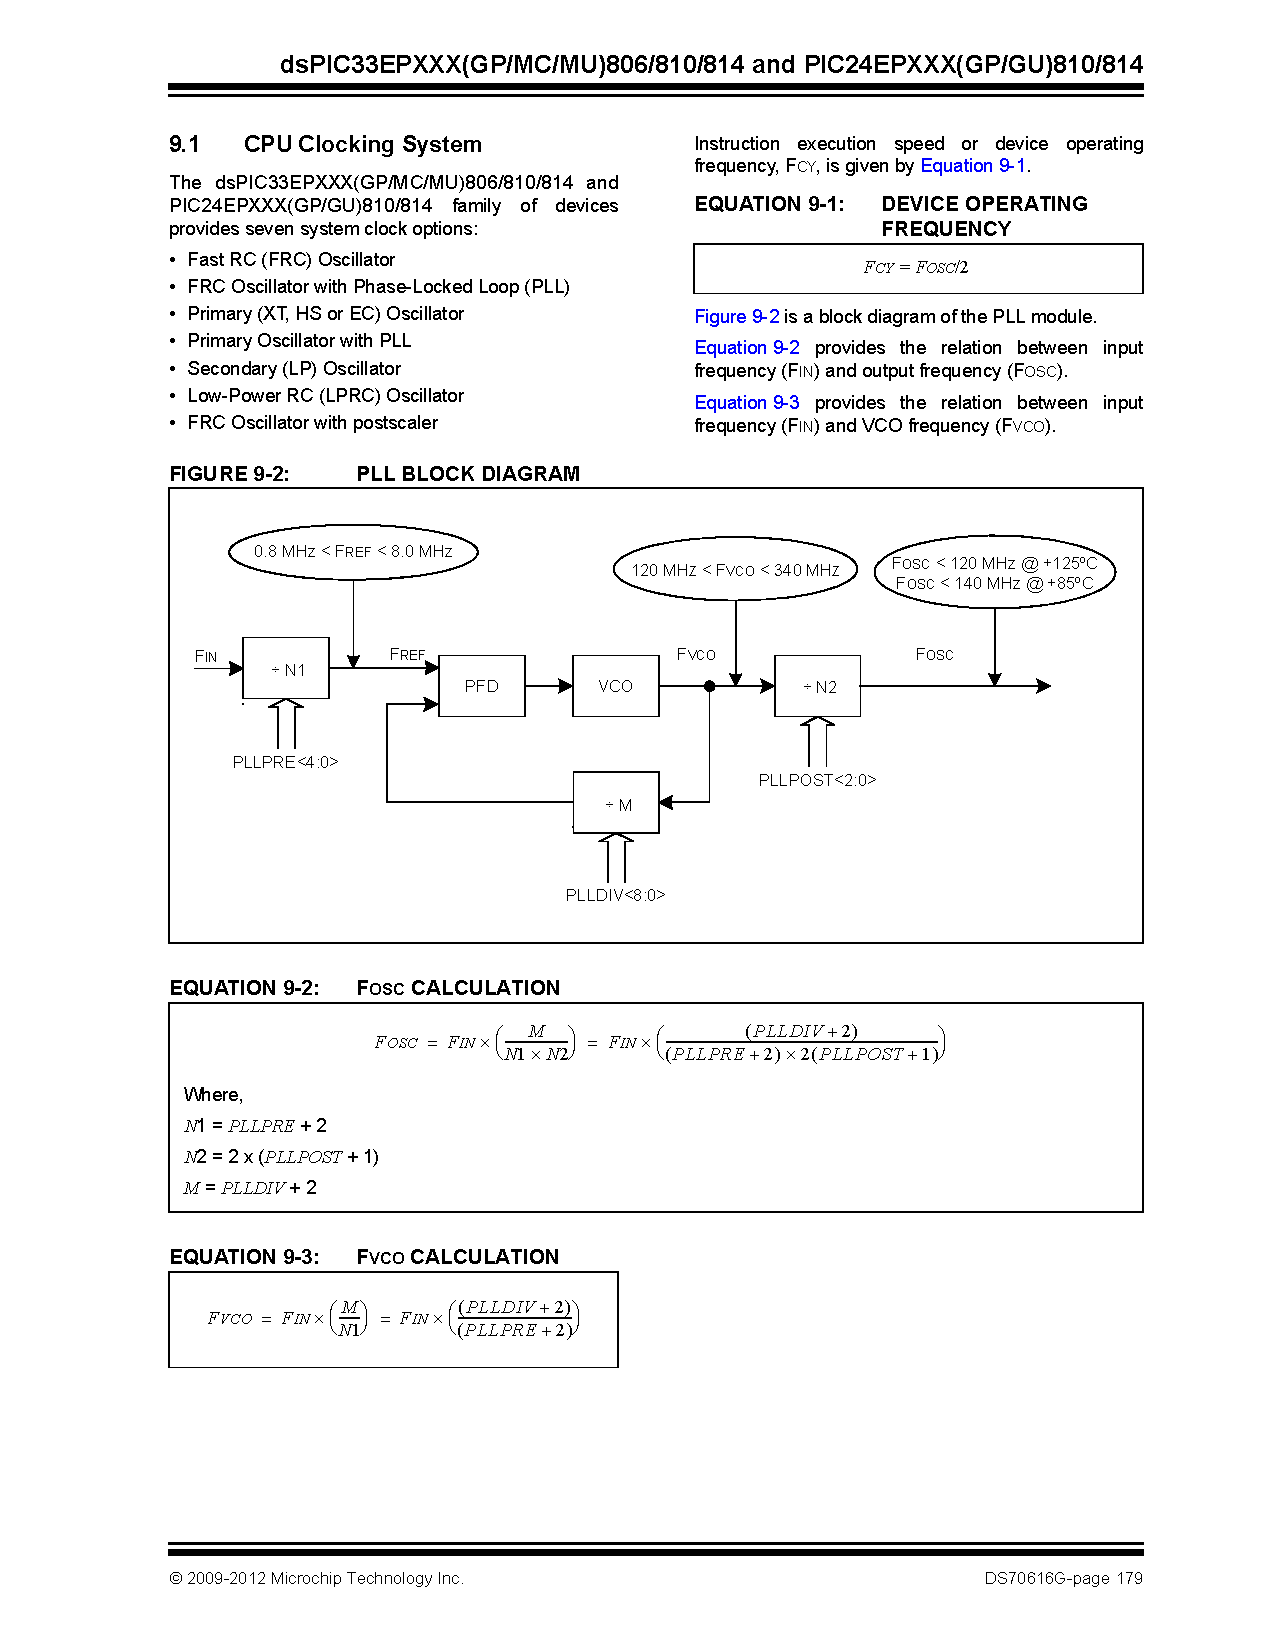
\includegraphics[width=\textwidth]{Images/CPUClockingSystem}
	\caption[CPU Blocking System]{CPU Clocking System mit PLL Block Diagramm}
	\label{image:CPUClockingSystem}
\end{figure}

\begin{figure}
	\centering
	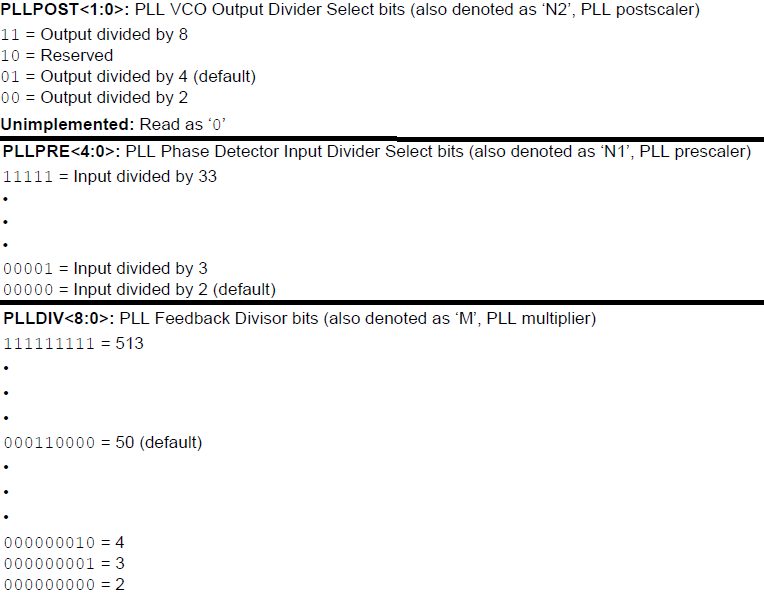
\includegraphics[width=\textwidth]{Images/PLLParameter}
	\caption[Wertebereich der PLL Parameter]{Wertebereich der PLL Parameter}
	\label{image:PLLParameter}
\end{figure}

\begin{figure}
	\centering
	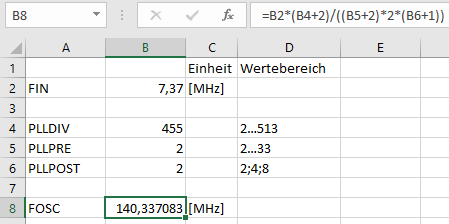
\includegraphics[width=0.95\textwidth]{Images/PLLParameterExcel}
	\caption[Berechnung der PLL Parameter in Excel]{PLL Parameter Excel}
	\label{image:PLLParameterExcel}
\end{figure}

\newpage
\begin{lstlisting}[frame=htrbl, caption={Code Example for Using PLL with 7.37 MHz Internal FRC}, label={lst:OscillatorSetup}]
// Select Internal FRC at POR
_FOSCSEL(FNOSC_PRIPLL); //Initial Oscillator: Primary Oscillator (XT, HS, EC) with PLL
_FOSC(POSCMD_HS);  //HS Crystal Oscillator Mode

int main()
{
// Configure PLL prescaler, PLL postscaler, PLL divisor
PLLFBD=455; // PLLDIV
CLKDIVbits.PLLPOST=2;
CLKDIVbits.PLLPRE=2;

// Wait for PLL to lock
while (OSCCONbits.LOCK!= 1);


while(1)
{
//endless loop
}

return 1; //never reached
}
\end{lstlisting}

\newpage

\section{Rechenleistung}
\subsection{Aufgabenstellung}

\begin{enumerate}%Aufzählung mit Numerierung
		\item Ermitteln Sie die durchschnittliche Laufzeit einschließlich Streuung arithmetischer Grundoperationen für verschiedene vom XC-16-Compiler unterstützten Datentypen. Wie erklären Sie die Unterschiede?
		\item Berechnen Sie die ersten 10 Primzahlen, die größer als 1.000.000 (1E6) sind. Implementieren Sie denselben Algorithmus auf einem PC und vergleichen Sie die Rechenzeiten.
		
\end{enumerate}

\subsection{Lösung}
\begin{enumerate}
		\item 
		Der Programmcode wird so umgeändert wie in Listening  \ref{lst:Rechenleistung} zu sehen. Zuerst wird mit dem Oszi nur die Zeit gemessen wie lange eine LED aus ist (ohne Rechenoperation, $29,1 ns$). Anschließend kann man mit dem Oszi messen wie lange eine Grundoperation (mit Zufallszahlen) inklusiv LED ein/ausschalten benötigt. Die folgende Auflistung beinhaltet nur die Zeitdauer für die jeweilige Rechenoperation (ohne LED ein/aus).\newline
\begin{tabular}{|c|c|c|c|c|c|c|}
	\hline 
	Datentyp & Operation & Zeitdauer &  & Datentyp & Operation & Zeitdauer \\
	\hline
	
	\hline
	uint8\_t 	& + & 43,7 ns &  		& int8\_t 		& + & 57,4 ns \\ 
	\hline 
				& - & 58,1 ns &  		&  				& - & 57,4 ns \\ 
	\hline 
				& * & 72,1 ns &  		&  				& * & 71,9 ns \\ 
	\hline 
				& / & 72,5 ns &  		&  				& / & 343,9 ns \\ 
	\hline 

	%&  &  &  &  &  &  \\ %empty Line 
	\hline 
	uint16\_t 	& + & 43,4 ns &  		& int16\_t 		& + & 43,3 ns \\ 
	\hline 
				& - & 43,5 ns &  		&  				& - & 43,4 ns \\ 
	\hline 
				& * & 86,2 ns &  		&  				& * & 87,4 ns \\ 
	\hline 
				& / & 330,9 ns &  		&  				& / & 329,9 ns \\ 
	\hline

	%&  &  &  &  &  &  \\ %empty Line 
	\hline 
	uint32\_t 	& + & 115,4 ns &  		& int32\_t 		& + & 142,9 ns \\ 
	\hline 
				& - & 114,9 ns &  		&  				& - & 112,9 ns \\ 
	\hline 
				& * & 245,9 ns &  		&  				& * & 230,9 ns \\ 
	\hline 
				& / & 7,559 us &  		&  				& / & 7,95 us \\ 
	\hline

	%&  &  &  &  &  &  \\ %empty Line 
	\hline 
	uint64\_t 	& + &  &  		& int64\_t 		& + & 254,9 ns \\ 
	\hline 
				& - &  &  		&  				& - & 226,9 ns \\ 
	\hline 
				& * &  &  		&  				& * & 1,5 us \\ 
	\hline 
				& / &  &  		&  				& / & 131 us \\ 
	\hline

	%&  &  &  &  &  &  \\ %empty Line 
	\hline 
	float 	& + &  &  				& long double 		& + &  \\ 
	\hline 
			& - &  &  		&  							& - &  \\ 
	\hline 
			& * &  &  		&  							& * &  \\ 
	\hline 
			& / &  &  		&  							& / &  \\ 
	\hline  
\end{tabular} 			
\newpage

		\item Der geforderte Algorithmus ist in Listening \ref{lst:Primzahlen} abgebildet. Bei dem verfügbaren Computer (Intel Core i7 2.6GHz, 16GB RAM, 64Bit Windows 10) ergab sich eine Laufzeit von ungefähr $5 us$. (Gemessen mit CodeBlocks, $50 s$ für $10^7$ Durchläufe)
		
		Die Laufzeit des selben Programms (angepasst auf die Hardware) benötigte auf dem Mikrocontroller Board $47,8 ms$. Der Code hierzu ist in Listing \ref{lst:PrimzahlenuC} abgebildet.
		
		Damit ist der Computer ca 10.000 mal schneller als der µC.
		 ($\frac{47,8 ms}{5 us} = 9560 $, Abbildung \ref{image:scopePrimzahlen}).
\end{enumerate}

\begin{figure}[h]
	\centering
	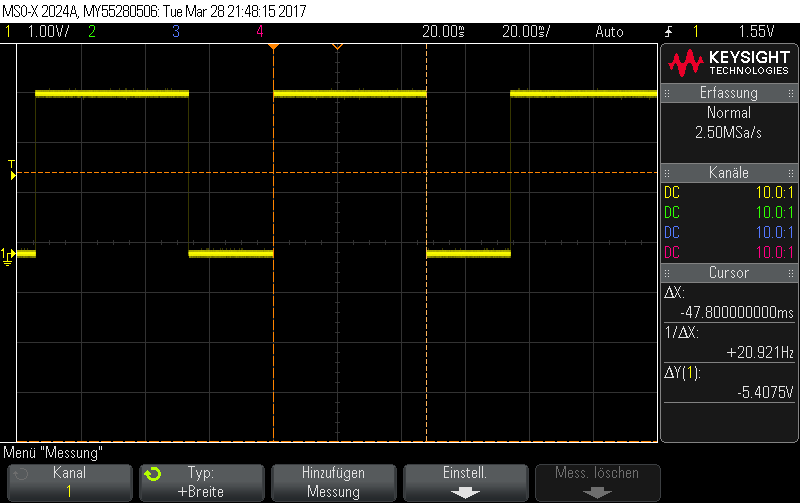
\includegraphics[width=\textwidth]{Images/scope_primzahlen}
	\caption[Laufzeit der Primzahlenberechnung]{Laufzeit der Primzahlenberechnung}
	\label{image:scopePrimzahlen}
\end{figure}

\newpage
\begin{lstlisting}[frame=htrbl, caption={Bestimmen der Rechenleistung}, label={lst:Rechenleistung}]
/* Endless Loop */
while(1){
_LED200=0;
ui8Var1 *= ui8Var2;
_LED200=1;
}//while
\end{lstlisting}

\begin{lstlisting}[frame=htrbl, caption={Algorithmus zur Berechnung der ersten 100 Primzahlen größer als 1E6}, label={lst:Primzahlen}]
#include<stdint.h>
#include<stdlib.h>
#include<math.h>

uint8_t isPrim(uint32_t ui32Number);

int main()
{
	uint32_t ui32Number= 1e6;  //start value
	uint16_t ui8PrimeCounter=0; //counts the number of calculated prime numbers
	const uint16_t ui8PrimMax=100;

	for(; ui8PrimeCounter<ui8PrimMax; ui32Number++)
		if(isPrim(ui32Number)) //check if the number is prime
		{
		//printf("%d\t%d\n",ui8PrimeCounter,ui32Number);
		ui8PrimeCounter++; //increase PrimeCounter, if the number is prime
		}
	return 0;
}
uint8_t isPrim(uint32_t ui32Number){
	uint32_t ui32Divider;
	uint32_t ui32SqrtNumber =((uint32_t) sqrt((double)(ui32Number)))+1;
	for(ui32Divider=2; ui32Divider<ui32SqrtNumber; ui32Divider++)
	{
		if((ui32Number%ui32Divider) == 0)
		{
			return 0; //uiNumber32 isn't a prime number
		}
	}
	return 1; //ui32Number is a Prime Number
}
\end{lstlisting}

\begin{lstlisting}[frame=htrbl, caption={Algorithmus zur Berechnung der ersten 100 Primzahlen größer als 1E6 auf dem uC}, label={lst:PrimzahlenuC}]
int main() {    //scope_25 47,8ms
	
	PLLFBD = 418;
	CLKDIVbits.PLLPOST = 2;
	CLKDIVbits.PLLPRE = 2;
	
	/* Port Configurations */
	// DS70616G-page 209
	// ODCB (open drain config) unimplemented (DS70616G, Table 4-56)
	ANSELBbits.ANSB8=0;     //Digital I/O
	CNENBbits.CNIEB8=0;     //Disable change notification interrupt
	CNPUBbits.CNPUB8=0;     //Disable weak pullup
	CNPDBbits.CNPDB8=0;     //Disable weak pulldown
	TRISBbits.TRISB8=0;     //Pin B8: Digital Output
	LATBbits.LATB8=0;       //Pin B8: Low
	_LED200 = 1;
	//uint32_t    ui32Var1=2;
	//uint32_t    ui32Var2=2;
	//uint32_t    ui32Var3=2;
	while (OSCCONbits.LOCK!= 1);
	/* Endless Loop */
	
	uint32_t ui32Number= 1000000;     //start value
	uint16_t ui8PrimeCounter=0;       //counts the number of calculated prime numbers
	const uint16_t ui8PrimMax=10;
	
	while(1){
		
		_LED200=1;      //hard on/off 28,5ns  scope_15
		
		ui32Number= 1000000;     //start value
		ui8PrimeCounter=0;       //counts the number of calculated prime numbers
		//ui8PrimMax=10;
		
		for(; ui8PrimeCounter<ui8PrimMax; ui32Number++)
		if(isPrim(ui32Number)) //check if the number is prime
		{
			//printf("%d\t%d\n",ui8PrimeCounter,ui32Number);
			ui8PrimeCounter++; //increase PrimeCounter, if the number is prime
		}
		
		_LED200=0; 
		delay_ms(500);
		
	}//while
	
	return (EXIT_SUCCESS);  //never reached
} //main()

uint8_t isPrim(uint32_t ui32Number){
	
	if(ui32Number==0 || ui32Number==1)
	return 0;
	
	
	if((ui32Number%2)==0)
	{
		if(ui32Number==2)
		{
			return 1;
		}
		else
		{
			return 0;
		}
	}
	uint32_t ui32Divider;
	uint32_t ui32SqrtNumber =((uint32_t) sqrt((long double)(ui32Number)))+1;
	
	for(ui32Divider=3; ui32Divider<ui32SqrtNumber; ui32Divider+=2)
	{
		if((ui32Number%ui32Divider) == 0) //check if ui32Divider is a in whole divider of ui32Number
		{
			return 0; //uiNumber32 isn't a prime number
		}
	}
	return 1; //ui32Number is a Prime Number
}
\end{lstlisting}
\newpage

\section{IO-Bibliothek}
\subsection{Aufgabenstellung}
Die populäre Arduino-Plattform (\url{https://www.arduino.cc/en/Reference/}) 
kapselt die Pinkonfiguration und -ansteuerung mit folgenden Funktionen:
\begin{itemize}
\item pinMode()
\item digitalRead()
\item digitalWrite()
\end{itemize}
Übertragen Sie dieses Konzept auf das EDA-Board. Anwendungsbeispiele:
\begin{itemize}
\item pinMode(SW1, IPUT\_PULLUP)
\end{itemize}
soll den Pin, an den SW1 angeschlossen ist, als digitalen Eingang konfigurieren und den Pullup-Widerstand einschalten.
\begin{itemize}
	\item digitalWrite(LED203, HIGH)
\end{itemize}
soll an dem Pin, an den LED203 angeschlossen ist,
einen High-Pegel ausgeben.
Verwenden Sie die Bezeichner aus dem Schaltplan.
Modularisieren Sie Ihre Software, verwenden Sie dazu die Dateinamen \textit{edaPIC33Hardware.h} und \textit{edaPIC33Hardware.c}.\newline \newline
Dokumentieren Sie die Funktionen mit Doxygen.\newline \newline
Messen Sie die Zeit, die zur Ansteuerung eines Ausgangspins mit den IO-Bibliotheksfunktionen notwendig ist
und vergleichen Sie diese mit einem direkten Schreiben in die entsprechenden Hardwareregister.

\subsection{Lösung}
Alle Device-Pins (ausgenommen VDD, VSS, MCLR and OSC1/CLKI) sind aufgeteilt auf die Ports für Peripheriegeräte und parallel I/O Ports. Alle I/O Ports sind Schmitt-Trigger Input (verbesserte Störungsunempfindlichkeit / Rauschempfindlichkeit).\newline
Alle Port Pins besitzen acht Register, durch diese Register lässt sich der I/O Port wie in Tabelle \ref{tab:ioports} dargestellt konfigurieren. Die Register Maps sind in Abbildung \ref{image:PORTA}-\ref{image:PORTG} dargestellt.\newline\newline
Ein Beispiel wie auf die einzelnen Register Bits zugegriffen werden kann und wie ein Port konfiguriert werden kann ist in Listing \ref{lst:confregport} zu sehen.\newline\newline
Die relevanten Auszüge aus dem Datenblatt sind in den Abbildungen \ref{image:page207}-\ref{image:page209} abgebildet.\newline\newline
Es wurde die Bibliothek mit den Dateien \textit{edaPIC33Hardware.h} und \textit{edaPIC33Hardware.c} erstellt. Die Funktion wurde mit Doxygen dokumentiert (TODO Anhang...).

\newpage
\begin{table}
\begin{tabular}{|l|l|}
	\hline 
	\textbf{Register Bit} & \textbf{Function}\\ 
	\hline
	TRISx 	&determines whether the pin is an input 	or an output\\
			&0:=output, 1:=input\\
			&default: all port pins are defined as inputs after a reset\\
	\hline 
	PORTx 	&read reads the port, write writes the latch \\ 
	\hline 
	LATx 	&read reads the latch, write writes the latch \\ 
	\hline 
	ODCx 	&configures pin for digital or open-drain output \\
			&0:=digital output, 1:=open drain output\\
	\hline 
	CNENx 	&enables change notification (CN) interrupts\\
			&0:=interrupts disabled, 1:=interrupts enabled\\
	\hline 
	CNPUx 	&enables weak pullup\\
			&0:=pullup disabled, 1:=pullup enabled\\  
	\hline 
	CNPDx 	&enables weak pulldown\\
			&0:=pulldown disabled, 1:=pulldown enabled\\  
	\hline 
	ANSELx 	&controls the operation of the analog port pins\\
			&0:=port operates as digital I/O port\\
			&1:=port operates as analog I/O port\\
	\hline
	note 	&Any bit and its associated data and control registers that are not\\
			&valid for a particular device is disabled. This means the correspon\\
			&-ding LATx and TRISx registers and the port pin are read as zeros.\\
	\hline
	note	&The open-drain feature allows the generation of outputs higher\\
			&than VDD (e.g., 5V on a 5V tolerant pin) by using external pull-up\\
			&resistors. The maximum open-drain voltage allowed is the same as \\
			&the maximum VIH specification for that pin.\\
	\hline
	note	&Pull-ups and pull-downs on change notification (CN) pins should\\
			&be disabled when the port pin is configured as a digital output.\\
	\hline
\end{tabular}
\caption{Konfigurationsmöglichkeiten der I/O Ports}
\label{tab:ioports}
\end{table}

\begin{lstlisting}[frame=htrbl, caption={Konfigurieren des Ports RB8 als Digitaler Input mit Pullup Widerstand}, label={lst:confregport}]
//configure RB8 as digit input with pullup
TRISBbits.TRISB8=1;     //configure as input
ANSELBbits.ANSB8=0;     //configure as digital
CNENBbits.CNIEB8=0;     //disable change notification interrupt
CNPUBbits.CNPUB8=1;     //enable weak pullup
CNPDBbits.CNPDB8=0;     //disable weak pulldown
\end{lstlisting}




\newpage

\section{Timer-Konfiguration}
\label{sec:Timer-Konfiguration} %label erstellen für quervereise
\subsection{Aufgabenstellung}
Konfigurieren Sie Timer 1 als freilaufenden Timer. Implementieren Sie eine Software-PWM:
\begin{itemize}
	\item Erzeugen Sie ein Ausgangssignal mit einer Frequenz von 1 kHz. Messen Sie das Signal mit dem Oszilloskop.
	\item Schreiben Sie ein Programm, das ein pulsweitenmoduliertes Signal mit einer Periodendauer von 1 ms (ggfs. 10 ms) und einem einstellbaren Tastverhältnis ausgibt.
	\item Erzeugen Sie damit ein PWM-Signal, dessen Gleichanteil einen dreieckförmigen Verlauf (Frequenz ca. 1 Hz) hat.
	\item Steuern Sie mit diesem Signal eine Leuchtdiode an
\end{itemize}
Optional: Ändern Sie das Programm "Hallo World"\ so ab, dass das Blinken der LED durch zyklisches Lesen des Timer1-Registers gesteuert wird.


\subsection{Lösung}
Das Timer1 Module ist ein 16-bit Timer (Zähler der mit einer konfigurierbaren Frequenz inkrementiert wird), welcher in folgenden Betriebsarten betrieben werden kann:
\begin{itemize}
	\item Timer mode
	\item Gated Timer mode
	\item Synchronous Counter mode
	\item Asynchronous Counter mode
\end{itemize}
Die restlicher Timer (2-8) sind jeweils als 16-bit single Timer, oder als 32-bit Timer konfigurierbar. Bei den 32-bit Timern werden immer zwei Timer (2/3,4/5,6/7,8/9) zusammengefasst. Zur Konfiguration siehe Datenblatt.
\newline
Die Konfigurationsmöglichkeiten der Timer sind in Tabelle \ref{tab:timermodesettings} abgebildet, das Blockdiagramm in Abbildung \ref{image:Timer1BlockDiagramm}.\newline
\begin{table}[h]
	\centering
	\begin{tabular}{|c|c|c|c|c|}
		\hline 
		\textbf{Mode} & \textbf{TCS} & \textbf{TGATE} & \textbf{TSYNC} & \multicolumn{1}{|c|}{Clock} \\ 
		\hline 
		\multicolumn{1}{|l|}{Timer} & 0 & 0 & X&$\frac{F_{OSC}}{2}$\\ 
		\hline 
		\multicolumn{1}{|l|}{Gated Timer}  & 0 & 1 & X&$\frac{F_{OSC}}{2}$ \\ 
		\hline 
		\multicolumn{1}{|l|}{Synchronous Timer} & 1 & X & 1& T1CK pin \\ 
		\hline 
		\multicolumn{1}{|l|}{Asynchronous Timer} & 1 & X & 0& T1CK pin\\ 
		\hline 
	\end{tabular} 
	\caption{Timer Mode Settings}
	\label{tab:timermodesettings}
\end{table}
\newline Die Konfiguration von Timer1 ist in Listening \ref{lst:Timer1Conf} zu sehen. Hierbei wurde Timer1 als freilaufender Timer1 konfiguriert. Durch zyklisches Abfragen der Werte von TMR1 kann man verschiedene Zeitdifferenzen bestimmen. Die Anzahl der Inkrements pro Sekunde berechnet sich zu:
\begin{equation}\label{key}
f_{inc}=\frac{F_{OSC}}{2*Prescaler}
\end{equation}
Die Anzahl der Inkrements die man für eine bestimmte Zeitdauer benötigt berechnet sich zu:
\begin{equation}\label{key}
Inkrements=f_{inc}*t
\end{equation}
Somit benötigt man beispielsweise für 0.5ms: $0.5ms*\frac{140MHz}{2*64}≈547$ Inkrements.\newline \newline
Bevor man die Differenzen der Timerwerte ausrechnet muss man einen Typecast auf int16\_t vornehmen, durch die Interpretation als Zweierkomplemennt ist sichergestellt, das auch bei einem Überlauf des Timers die richtige Differenz berechnet wird. Ein Beispiel hierzu ist in Listening \ref{lst:Timer1OnCycle} zu sehen.
\newline Der Tastgrad ist auch variabel eingestellt, wie in Listing \ref{lst:Timer1OnCycle} zu sehen toggelt der digitale Ausgang immer zwischen HIGH und LOW, abhängig von der Anzahl an "dT"\ Increments (siehe if-Abfragen).


\begin{lstlisting}[frame=htrbl, caption={Timer1 Configuration}, label={lst:Timer1Conf}]
T1CONbits.TON = 0; // Disable Timer
//set the multiplexer to timer mode
T1CONbits.TCS = 0;   // Select internal instruction cycle clock
T1CONbits.TGATE = 0; // Disable Gated Timer mode

T1CONbits.TCKPS = 0b10; // Select 1:64Prescaler

TMR1 = 0x00; // Clear timer register
PR1 = 0xFFFF; // Load the period value

//disable interrupt
IPC0bits.T1IP = 0x00;// Set Timer 1 Interrupt Priority Level
IFS0bits.T1IF = 0; // Clear Timer 1 Interrupt Flag
IEC0bits.T1IE = 0; // Enable Timer1 interrupt 

T1CONbits.TON = 1; // Start Timer
\end{lstlisting}

\begin{lstlisting}[frame=htrbl, caption={Timer1 on Cycle}, label={lst:Timer1OnCycle}]
int16_t    _i16Timer1_1kHz_dTOn=0;
int16_t    _i16Timer1_1kHz_dTOff=0;
uint8_t    _ui8Timer1_1kHz_Port=0;

void onCycleTimer1PWM_1kHz()
{
	static uint8_t _ui8Timer1_1kHz_Mode=0;
	static int16_t _i16Timer1_1kHz_T0 = 0;
	int16_t i16_T1 = (int16_t)TMR1;
	if(_ui8Timer1_1kHz_Mode == 0)
	{
		if((i16_T1 - _i16Timer1_1kHz_T0) >= _i16Timer1_1kHz_dTOff) //_i16Timer1_1kHz_dTOff
		{
			digitalWrite(_ui8Timer1_1kHz_Port,HIGH);
			_i16Timer1_1kHz_T0 = (int16_t)TMR1;
			_ui8Timer1_1kHz_Mode=1;        
		}
	}
	else
	{
		if((i16_T1 - _i16Timer1_1kHz_T0) >= _i16Timer1_1kHz_dTOn) //_i16Timer1_1kHz_dTOn
		{
			digitalWrite(_ui8Timer1_1kHz_Port,LOW);
			_i16Timer1_1kHz_T0 = (int16_t)TMR1;
			_ui8Timer1_1kHz_Mode=0;       
		}

	}  	
}
\end{lstlisting}

\begin{figure}[h]
	\centering
	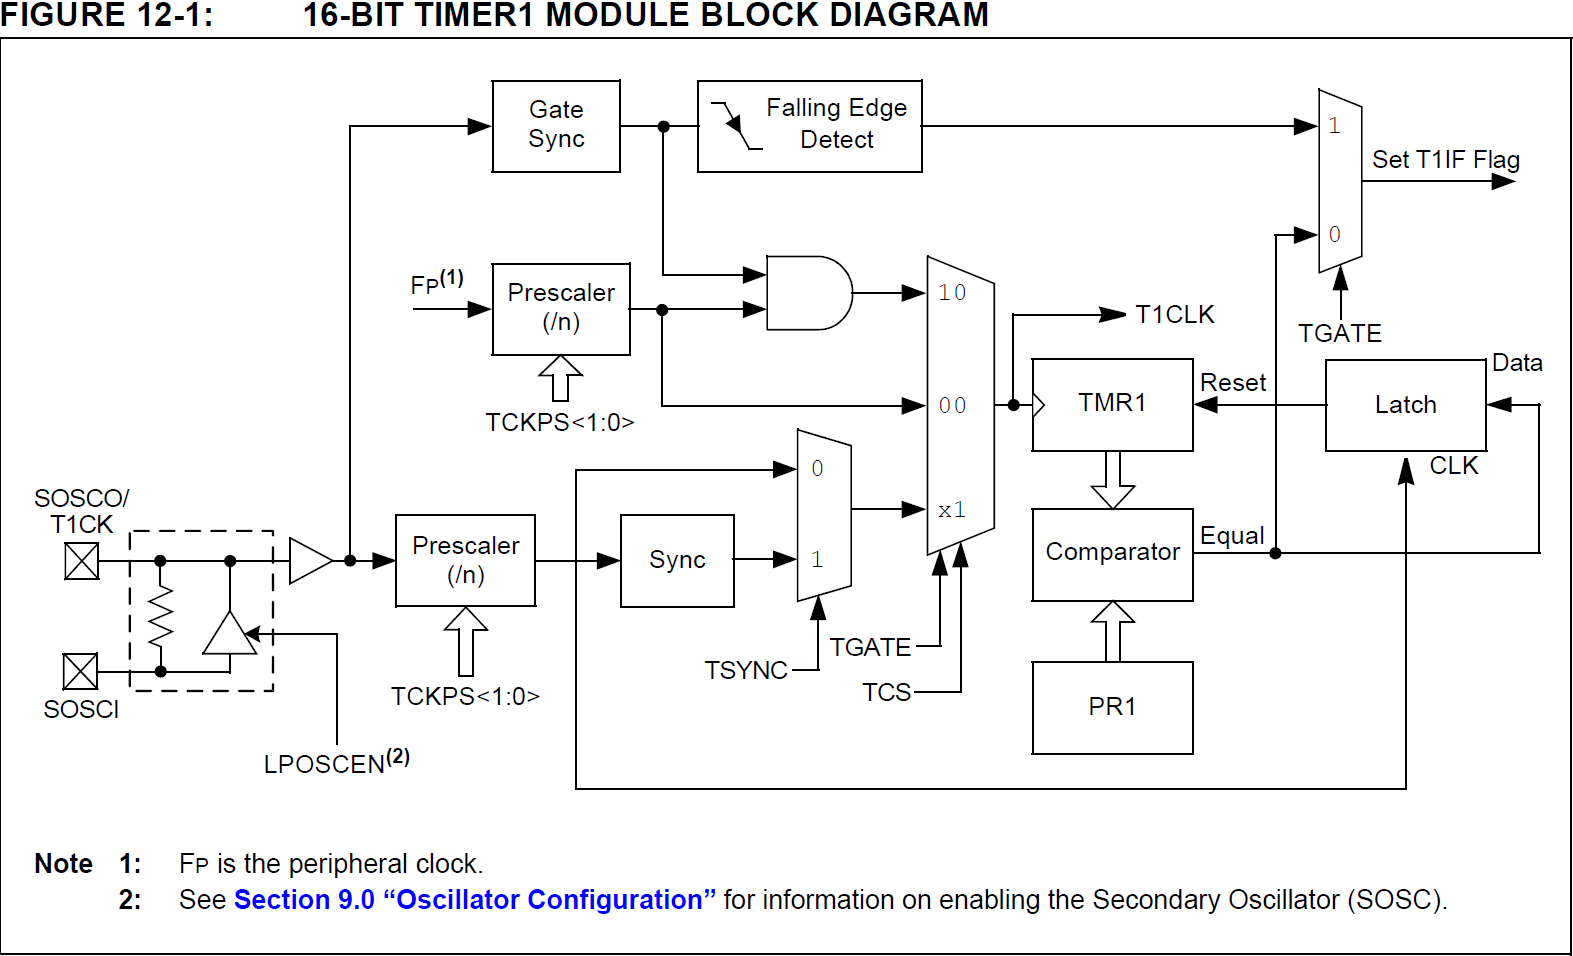
\includegraphics[width=\textwidth]{Images/timer1blockdiagramm}
	\caption[Timer1 Block Diagramm]{Timer1 Block Diagramm}
	\label{image:Timer1BlockDiagramm}
\end{figure}

\newpage

\section{SystemTime}
\subsection{Aufgabenstellung}

Schreiben Sie ein Modul mit folgender Funktionalität:
\begin{itemize}
	\item getSystemTimeMillis()
\end{itemize}
Die genannte get-Funktion soll den Wert eines Zählers liefern, welcher in der Timer-1-ISR jede Millisekunde inkrementiert wird. Der Zähler selbst soll außerhalb des Moduls nicht sichtbar sein.
Innerhalb des Moduls soll auch der Timer konfiguriert werden.\newline
Testen Sie das Modul mit einem Programm, das mittels getSystemTimeMillis() ein Rechtecksignal mit einer Frequenz von 50 Hz und einer Einschaltdauer von 25\% generiert.\newline\newline
Hinweise zur Implementierung:\newline
Beachten Sie, dass ein Interrupt auch eine 32-Bit-Leseoperation unterbrechen kann. Entwickeln Sie einen Mechanismus, mit dem  getSystemTimeMillis() auch in diesem Fall einen konsistenten Zählerstand zurückliefert.\newline\newline
{\footnotesize Ergänzung:\newline
Konfigurieren Sie Timer 3 in Verbindung mit dem 32-kHz-Quarz so, dass jede Sekunde ein Interrupt ausgelöst wird. Schreiben Sie in gleicher Weise wie oben eine Funktion getSystemTimeSeconds()
Testen Sie die Funktion, indem Sie damit eine LED im Zweisekundentakt blinken lassen.
}
\subsection{Lösung}
Die geforderte Funktion wurde durch die drei Funktionen aus Listing \ref{lst:SysTimeFunctions} realisiert. Die Funktion configSystemTimeMillis() konfiguriert Timer 1 als nicht freilaufenden Timer mit der Incrementfrequenz $ F_P=\frac{F_{OSC}}{2} $ und erlaubt Interrupts.\newline
In der Interrupt Service Routine (ISR) wird dann die globale Variable ui32SystemTimeMillis nach jedem ausgelöstet Interrupt erhöht.\newline
Bevor diese Variable in der getSystemTimeMillis() Funktion gelesen wird, wird ein globales Access Flag gesetzt (ui8SystemTimeMillisAccesFlag). Versucht man während eines Interrupts die Variable zu lesen, dann erkennt dies die ISR und setzt ein Kollisions-Flag (ui8SystemTimeMillisConflictFlag). Wurde eine Kollision erkannt, dann liefert getSystemTimeMillis() den zuletzt gespeicherten Wert zurück, so wird eine falscher Rückgabewert beim Lesen der ui32SystemTimeMillis-Variable während einem Interrupt vermieden.



%Beispiel für Quellcode Listening
\newpage
\begin{lstlisting}[frame=htrbl, caption={System Time Funktionen}, label={lst:SysTimeFunctions}]
void configSystemTimeMillis()
{
  T1CONbits.TON = 0; //Disable Timer
  T1CONbits.TCS = 0; //internal instruction cycle clock
  T1CONbits.TGATE = 0; // Disable Gated Timer mode
  T1CONbits.TCKPS = 0b01; // Select 1:8 Prescaler
  TMR1 = 0x00; // Clear timer register
  PR1 = 8750-1;  //Period Value: 140Mhz: 8750-1 / 120Mhz: 7500-1
  IPC0bits.T1IP = 0x01; //Timer 1 Interrupt Priority Lvl
  IFS0bits.T1IF = 0; // Clear Timer 1 Interrupt Flag
  IEC0bits.T1IE = 1; // Enable Timer1 interrupt
  T1CONbits.TON = 1; // Start Timer
}

uint32_t getSystemTimeMillis()
{
  uint32_t ui32ReturnValue=0;
  static uint32_t ui32OldValue=0; 
	
  ui8SystemTimeMillisAccesFlag = 1;
  ui32ReturnValue = ui32SystemTimeMillis;
  ui8SystemTimeMillisAccesFlag = 0;
	
  if(ui8SystemTimeMillisConflictFlag ==1)
  {
	ui8SystemTimeMillisConflictFlag=0;
	ui32ReturnValue =  ui32OldValue;
  }

  ui32OldValue = ui32ReturnValue;

  return ui32ReturnValue;
}

void __attribute__((__interrupt__, no_auto_psv)) _T1Interrupt(void) //Timer1 ISR
{
  ui32SystemTimeMillis++;  //increase millis counter
  if (ui8SystemTimeMillisAccesFlag == 1)    //if acces flag=1, set config flag
	ui8SystemTimeMillisConflictFlag = 1;
  else
	ui8SystemTimeMillisConflictFlag = 0;
	
  IFS0bits.T1IF = 0;      //Clear Timer1 interrupt flag
}
\end{lstlisting}


\newpage

\section{Non-blocking Code}
\subsection{Aufgabenstellung}
Schreiben Sie ein Programm mit folgender Funktionalität:
\begin{itemize}%Aufzählung mit Numerierung
		\item Die 4 LEDs auf dem Board sollen mit unterschiedlichen Periodendauern blinken: 2*300ms, 2*500ms, 2*700ms und 2*1100ms blinken.
		\item Zu wie viel Prozent ist die CPU ausgelastet?
		\item Die Leuchtdauer der LEDs soll per Tastendruck einstellbar sein. Genau die Zeitdauer, während der ein zugeordneter Taster gedrückt ist, definiert den Sollwert für die halbe Periodendauer.
\end{itemize}
Hinweise zur Implementierung:
\begin{itemize}
	\item Wenden Sie das Konzept des kooperativen Multitaskings (non-blocking Code) an.
	\item Verwenden Sie getSystemTimeMillis().
\end{itemize}

\subsection{Lösung}
Bei der Implementierung der geforderten Funktionen wurde davon ausgegangen, dass die Funktionen zyklisch jede ms aufgerufen werden. Somit können die Funktionen losgelöst von Timern implementiert werden.\newline
Die Funktion zum zyklischen blinken der LED sind in Listening \ref{lst:blinkLed} dargestellt. Die Funktion zum messen der ToggleTime sind in Listening \ref{lst:measuretoggletimesw0} dargestellt. \newline
Die Auslastung der CPU liegt bei ca. 1\%. In Listening \ref{lst:mainnonblocking} ist die main Funktion dargestellt, diese stellt sicher, dass alle Funktionen zyklisch jede ms aufgerufen werden.

\begin{figure}[h]
	\centering
	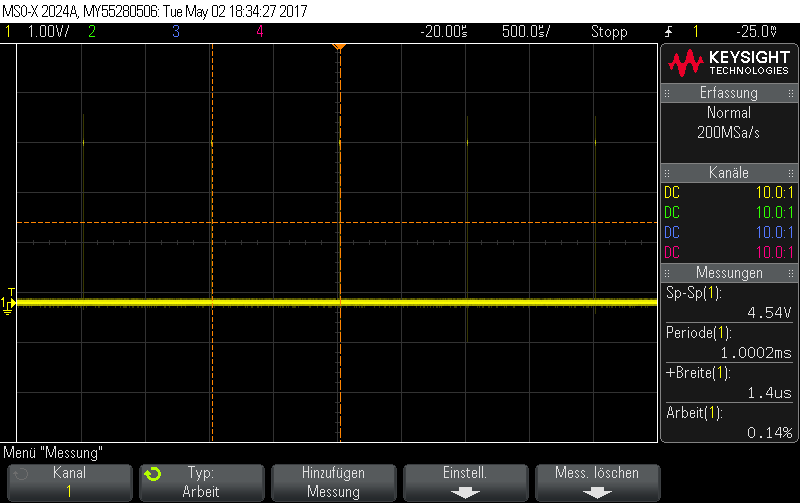
\includegraphics[width=0.7205\textwidth]{Images/scope_nonblockingcodepng}
	\caption[NonBlockingCode]{Auslastung der CPU}
	\label{image:nonblockingcode}
\end{figure}

\newpage
\begin{lstlisting}[frame=htrbl, caption={blinkLed0() Funktion}, label={lst:blinkLed}]
/** 
* @brief Toggle LED0 (RB_8) with toggle Time
* @param uint16_t ui16ToggleTime Toggle Time in Functions Calls
* @details Toggles RB_8 with the number of functions calls.
* @details Example: If Toggle Time is 20, you have to call the function 20 times to toggle RB_8
* @attention toggle pin has to be defined as digital output first
*/
void blinkLed0(uint16_t ui16ToggleTime)
{
  static uint16_t ui16Counter = 0;

  if(ui16ToggleTime == 0)
  {
    ui16Counter=0;
    digitalWrite(LED0,LOW);
    return;
  }
  else
    ui16Counter++;

  if(ui16Counter >= ui16ToggleTime)
  {
    ui16Counter=0;
    digitalToggle(LED0);
  }
}
\end{lstlisting}
\newpage
\begin{lstlisting}[frame=htrbl, caption={measureToggleTimeSW0() Funktion}, label={lst:measuretoggletimesw0}]
/** 
* @brief Measure hold Time from RG_12
* @returns uint16_t ui16HoldTime HoldTime is measured in function calls
* @details Measures Hold Time in Functions calls, if the Pin is not hold (high level) the functions retuns the last measured hold time
* @details Example: If the Pin is hold for 40ms you get the return value 40 when the function is called each ms, or the return value 20 when the function is called each 2ms
* @attention Pin has to be configured as input first, the functions is low active
*/
uint16_t measureToggleTimeSW0()
{
  static uint16_t ui16ToggleTime=0;
  static uint8_t  ui8MeasureMode=0;

  if(digitalRead(SW0)==LOW && (ui8MeasureMode==0))
  {
    ui16ToggleTime=0;
    ui8MeasureMode=1;
  }

  if(ui8MeasureMode==1)
  {
    ui16ToggleTime++;
  if(digitalRead(SW0)==HIGH)
    ui8MeasureMode=0;
  }

  return ui16ToggleTime;
}
\end{lstlisting}

\newpage
\begin{lstlisting}[frame=htrbl, caption={NonBlockingCode Main-Funktion}, label={lst:mainnonblocking}]
int main() {
	configOscillator();
	
	//set LED pinmodes
	pinMode(LED0,OUTPUT);
	pinMode(LED1,OUTPUT);
	pinMode(LED2,OUTPUT);
	pinMode(LED3,OUTPUT);
	
	//set switch pinmodes
	pinMode(SW0, INPUT_PULLUP);
	pinMode(SW1, INPUT_PULLUP);
	pinMode(SW2, INPUT_PULLUP);
	pinMode(SW3, INPUT_PULLUP);
	
	//config timer 1 for getSystemTimeMillis();)
	configSystemTimeMillis();
		
	/* Endless Loop */
	while(1){
		static uint32_t ui32Time= 0;
		
		blinkLed(LED0, measureToggleTimeSW(SW0));
		blinkLed(LED1, measureToggleTimeSW(SW1));
		blinkLed(LED2, measureToggleTimeSW(SW2));
		blinkLed(LED3, measureToggleTimeSW(SW3));
				
		ui32Time++; //increase ms counter
		while(getSystemTimeMillis() < ui32Time) //wait rest of 1ms
		{
			ClrWdt();   //clear watchdog timer
		}
	}//while
	return (EXIT_SUCCESS);  //never reached
} //main()
\end{lstlisting}


\newpage

\section{Software-Entwurf mit FSM}
\subsection{Aufgabenstellung}
\begin{enumerate}%Aufzählung mit Numerierung
		\item Entprellen der Taster
		\begin{itemize}
			\item Messen Sie die typische Prelldauer einer Taste mit dem Oszilloskop. Welche Entprellzeit schlagen Sie vor?
			\item Schreibe Sie eine Funktion \texttt{isPressed()}, mit der Tasteneingaben entprellt werden. 
		\end{itemize}
		\item LED mit einem Taster an- und ausschalten
		\begin{itemize}
			\item Eine LED soll mit einem Tastendruck angeschaltet und mit einem weiteren Tastendruck ausgeschaltet werden.
			\item Optional: Mit jedem Tastendruck soll eine LED aus- und die nächste angeschaltet werden.
		\end{itemize}
		\item Nachbildung eines Treppenlichtautomaten
		\begin{itemize}
			\item Auf Tastendruck geht das Licht (LED) an
			\item Das Licht bleibt für eine bestimmte (tbd.) Zeit an
			\item Anschließend wird das Licht kontinuierlich bis auf Null gedimmt
			\item Der Automat soll nachtriggerbar sein
		\end{itemize}
\end{enumerate}
Hinweise zur Implementierung:
\begin{itemize}
	\item Modellieren Sie die Funktionalität als FSM (Moore-Automat).
	\item Beachten Sie, dass das Debouncen (Entprellen) bei beiden Flankenwechseln stattfinden muss
\end{itemize}

\subsection{Lösung}
\begin{enumerate}
		\item Es wurden mehrere Prellvorgänge mit dem Oszilloskop gemessen. Je nach verwendetem Taster und der Art wie man den Taster drückt sind verschiedenen Prellvorgänge aufgenommen worden, diese sind in Abbildung \ref{image:prellen} dargestellt.\newline
		Die längste aufgenommene Prelldauer beträgt 250us. Ich wähle jedoch pauschal eine Entprelldauer (\grqq Debounce-Time\grqq) von $1ms$ vor, da durch vorherige Programmierschritte festgelegt wurde, dass der Mikrocontroller die \grqq Loop\grqq zyklisch im Takt von $1ms$ durchläuft.\newline
		Die Funktion \textit{isPressedSW0()} (Listening \ref{lst:ispressedsw0}) wurde als Zustandsautomat Implementiert. Die Funktion sollte zyklisch aufgerufen werden. Eine Skizze des Zustandsautomats ist in Abbildung \ref{image:statemachineispressed} zu sehen.
		\item Es wurde eine Funktion geschrieben, welche immer bei einem Tastendruck (Flanke von High auf Low) die LED toggled (Listening \ref{lst:FlipFlopLED0}).
		\item Der Treppenlichtautomat wurde ebenfalls als Zustandsautomat implementiert, von der Auflistung des Quellcodes wird aus Übersichtsgründen abgesehen.
\end{enumerate}



\begin{lstlisting}[frame=htrbl, caption={Funktion isPressedSW0()}, label={lst:ispressedsw0}]
#define STATE_STABLE_HIGH   0
#define STATE_INSTABLE_HIGH 1
#define STATE_STABLE_LOW    2
#define STATE_INSTABLE_LOW  3
const uint16_t cui16DebounceTime=1;


uint8_t isPressedSW0()
{
	static uint8_t ui8State = STATE_STABLE_HIGH; //default state
	static uint16_t ui16Counter=0;
	uint8_t ui8ReturnValue=1;
	
	switch(ui8State)
	{             
	case STATE_STABLE_HIGH:
		if(digitalRead(SW0)==LOW)
		{
			ui8State = STATE_INSTABLE_HIGH;
			ui16Counter=0;
		}
		ui8ReturnValue= HIGH;
	break;
	
	case STATE_INSTABLE_HIGH:
		ui16Counter++;
		if(digitalRead(SW0)==LOW)
		{
			if( ui16Counter>=cui16DebounceTime )
			{
				ui8State = STATE_STABLE_LOW;
				ui8ReturnValue= LOW;
			}
			else
				ui8ReturnValue= HIGH;
		}
		else
		{
			ui8State = STATE_STABLE_HIGH;
			ui8ReturnValue= HIGH;
		}
	break;
	
	case STATE_STABLE_LOW:
		if(digitalRead(SW0)==HIGH)
		{
			ui8State = STATE_INSTABLE_LOW;
			ui16Counter=0;
		}
		ui8ReturnValue= LOW;
	break;
	
	case STATE_INSTABLE_LOW:
		ui16Counter++;
		if(digitalRead(SW0)==HIGH)
		{
			if(ui16Counter >= cui16DebounceTime)
			{
				ui8State = STATE_STABLE_HIGH;
				ui8ReturnValue= HIGH;
			}
			else
				ui8ReturnValue= LOW;
		}
		else
		{
			ui8State = STATE_STABLE_LOW;
			ui8ReturnValue= LOW;
		}            
	break;
	
	default:
		ui8State = STATE_STABLE_HIGH;
		ui8ReturnValue= HIGH;
	break;
	}
	
	return ui8ReturnValue;
}
\end{lstlisting}




\begin{lstlisting}[frame=htrbl, caption={LED auf Tastendruck Toggeln}, label={lst:FlipFlopLED0}]
void FlipFlopLED0(uint8_t ui8SwitchState)
{
	static uint8_t ui8OldSwitchState = HIGH;
	
	if(ui8OldSwitchState == HIGH && ui8SwitchState == LOW) //Flanke von HIGH auf LOW
	{
		digitalToggle(LED0);
	}
	ui8OldSwitchState=ui8SwitchState;
}
\end{lstlisting}
\newpage
\begin{lstlisting}[frame=htrbl, caption={Funktion digitalCountLED0to3()}, label={lst:digitalCountLED0to3}]
void digitalCountLED0to3(uint8_t ui8SwitchState)
{
static uint8_t ui8OldSwitchState = HIGH;
static uint8_t ui8CountValue=0;

	if(ui8OldSwitchState == HIGH && ui8SwitchState == LOW) //Flanke von HIGH auf LOW
	{
		ui8CountValue++;
		digitalWrite(LED0, ui8CountValue&0x01);
		digitalWrite(LED1, ui8CountValue&0x02); 
		digitalWrite(LED2, ui8CountValue&0x04);
		digitalWrite(LED3, ui8CountValue&0x08);
	}
	ui8OldSwitchState=ui8SwitchState;
}
\end{lstlisting}
\newpage
%einbinden einer Grafik 
\begin{figure}[h!]
	\subfigure[Prellvorgang von ca $10us$]{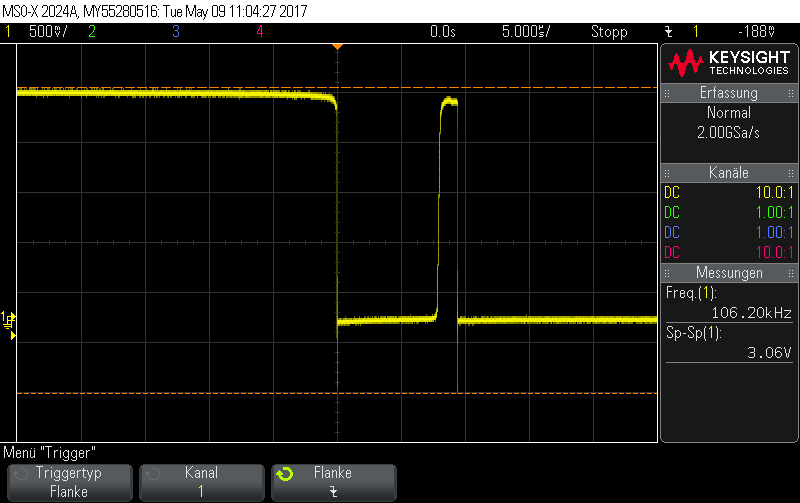
\includegraphics[width=0.49\textwidth]{Images/prellen1}} 
	\subfigure[Prellvorgang von ca $8ns$]{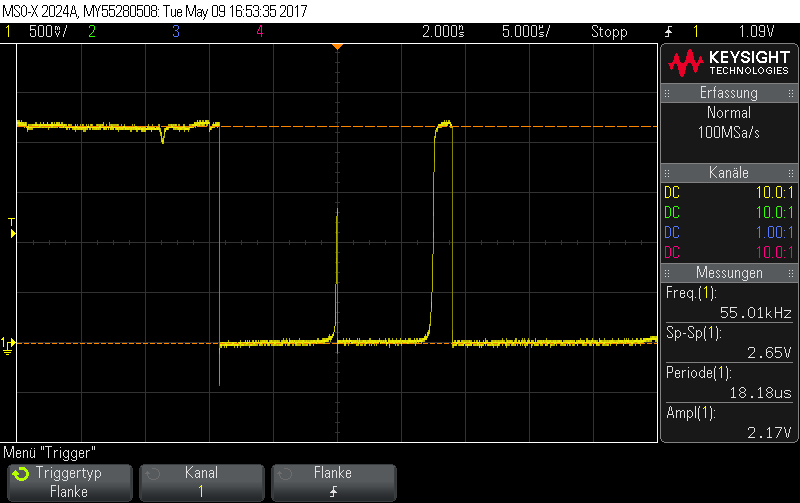
\includegraphics[width=0.49\textwidth]{Images/prellen2}} 
	%\caption{Titel unterm gesamten Bild}
	\subfigure[Prellvorgang von ca $6us$]{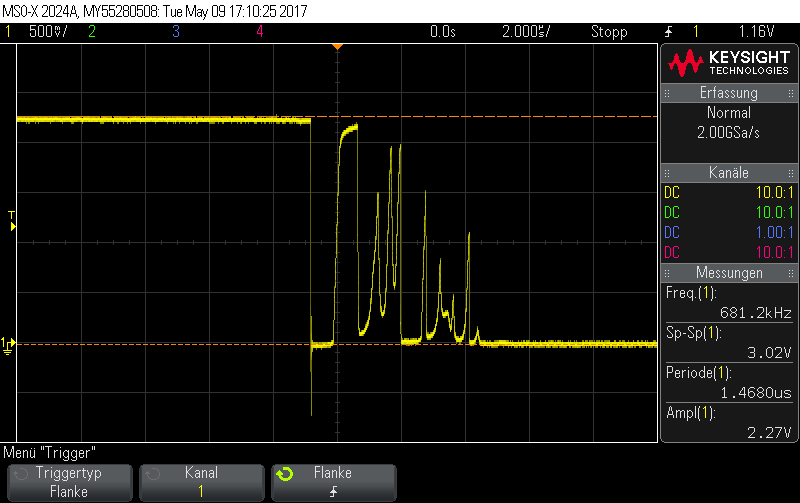
\includegraphics[width=0.49\textwidth]{Images/prellen3}} 
	\subfigure[Prellvorgang von ca $150us$]{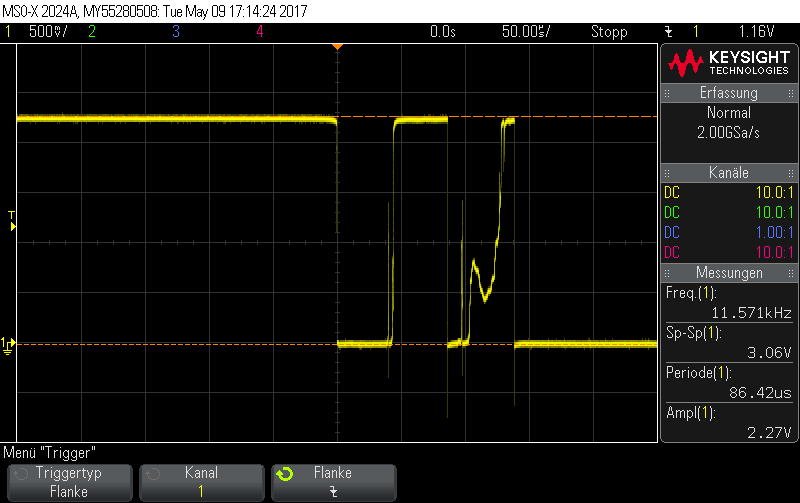
\includegraphics[width=0.49\textwidth]{Images/prellen4}} 
	%\caption{Titel unterm gesamten Bild} 
	\subfigure[Prellvorgang von ca $35us$]{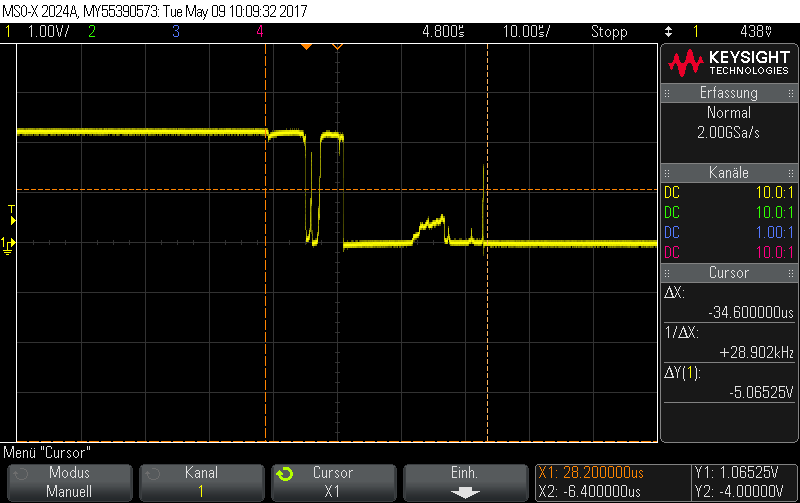
\includegraphics[width=0.49\textwidth]{Images/prellen5}} 
	\subfigure[Prellvorgang von ca $250us$]{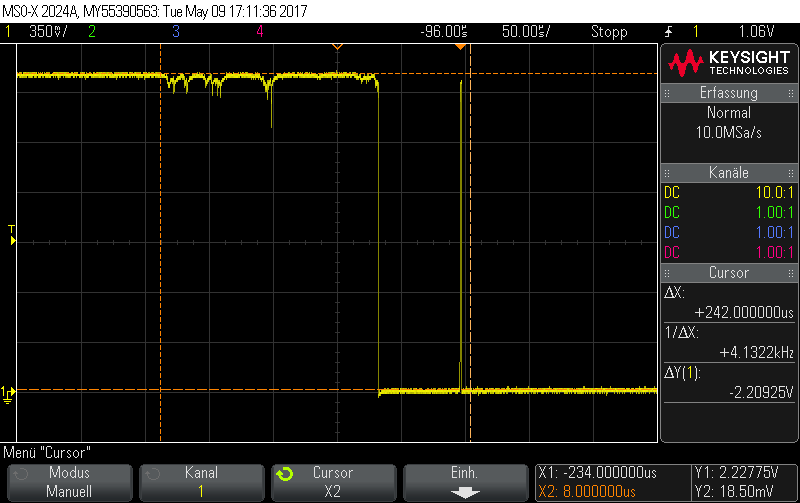
\includegraphics[width=0.49\textwidth]{Images/prellen6}} 
	\caption{Mehrere Prellvorgänge (entnommen aus Moodle)}
	\label{image:prellen}
\end{figure}

\newpage
\begin{figure}[h!]
	\centering
	\subfigure[Zeitliches Verhalten beim Prellen]{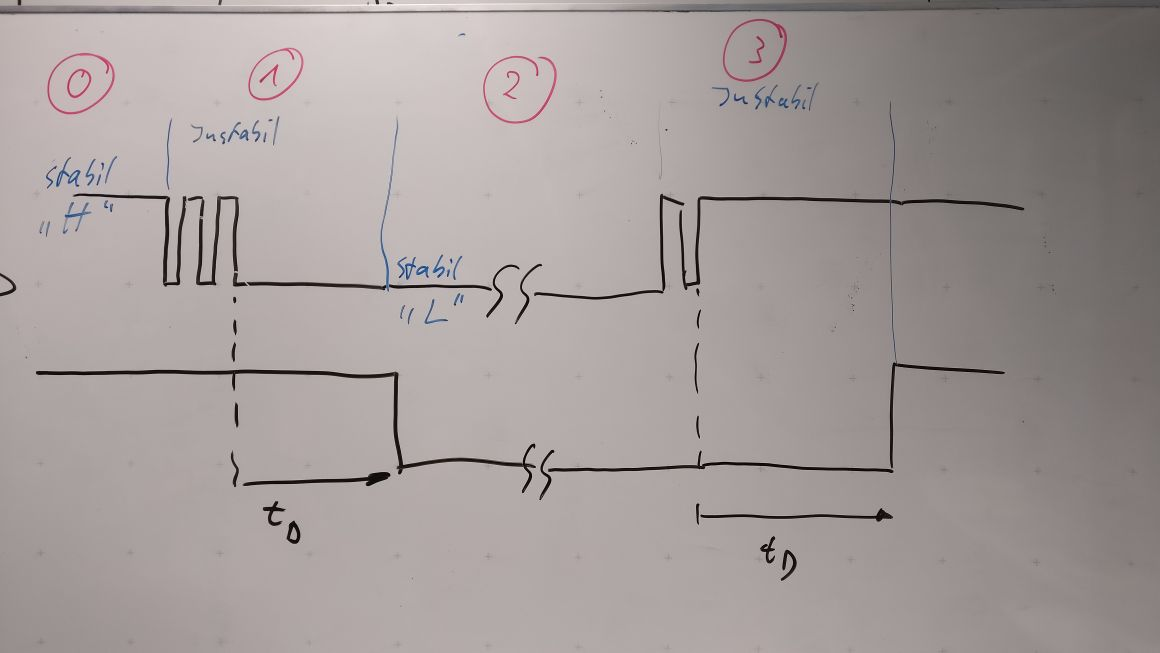
\includegraphics[width=\textwidth]{Images/statemachine2}} 
	\subfigure[Zustandsautomat]{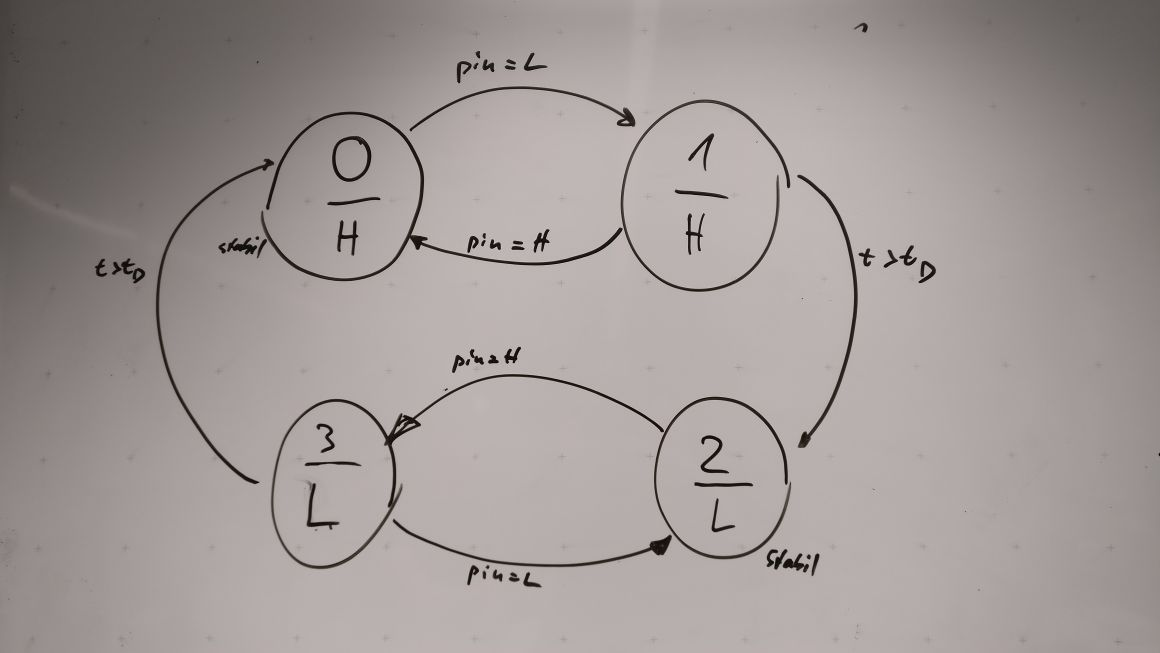
\includegraphics[width=\textwidth]{Images/statemachine}} 
	\caption[NonBlockingCode]{Skizzen zu der Funktion isPressed()}
	\label{image:statemachineispressed}
\end{figure}
\newpage
\newpage

\section{LCD-Bibliothek}
\subsection{Aufgabenstellung}
Schreiben Sie eine Bibliothek zur Ansteuerung des LC-Displays auf dem EDAdsPIC33-Board:
\begin{itemize}
	\item Initialisierung (blocking Code erlaubt)
	\item Zyklisches Kopieren eines Schattenspeichers in den Display-Speicher\newline
			(non-blocking code).
\end{itemize}

\subsubsection*{Hinweise zur Implementierung}

Literatur:
\begin{itemize}
	\item DiJasio(2012): Chapter 9\newline
			\url{https://www.dropbox.com/sh/4bwfkqux88a3j62/AAAhId8mi25vsYaToLJbrS1Ba?dl=0\&preview=09_Glass_Bliss.pdf}
	\item Datenblatt FDCC1602L-NSWBBW-91LE, \newline \url{http://farnell.com/datasheets/653662.pdf}
	\item Datenblatt Displaycontroller \newline
			\url{https://sparkfun.com/datasheets/LCD/HD44780.pdf}\newline
			\url{http://download.maritex.com.pl/pdfs/op/TC1602E-06H.pdf}
	\item Simulator \newline
	 \url{http://dinceraydin.com/djlcdsim/djlcdsim.html}
	
\end{itemize}

Vorgehensweise:
\begin{itemize}
	\item Schreiben Sie zunächst eine Funktion putLCD(), die ein Zeichen auf dem Display ausgibt (blocking code)
	\item Ändern Sie die Funktion so, dass sie kooperativ wird.
	\item Implementieren Sie anschließend das Kopieren des Schattenspeichers
\end{itemize}

\subsection{Lösung}

\begin{enumerate}
		\item Lösungsansatz 1
		\item Lösungsansatz 2
		\item Lösungsansatz 3
		\item Lösungsansatz 4
\end{enumerate}


%Beispiel für Quellcode Listening
\begin{lstlisting}[frame=htrbl, caption={Listening Bezeichnung}, label={lst:Referenzname}]
//Quellcode
\end{lstlisting}


\newpage

\section{Mitschrift aus Vorlesung}
\subsection{Vorlesung 04.04.2017 - IO-Bibliothek}

\begin{itemize}%Aufzählung mit Numerierung
		\item jeder uC is universell aufgebaut und muss für jeden Fall individuell konfiguriert werden
		\item kleine Bibliothek zum anpassen der IO-Ports ist praktisch
		\item Lese und Schreib Funktionalität soll realisiert werden
		\item Datenblatt Figure 11-1 -> Pins müssen über Treiber realisiert werden, Schmitt-Trigger ist enthalten
		\item Pegel um Treiber zu aktivieren? nachlesen Schaltbild könnte falsch sein
		\item Lesezugriff über Port, Schreibezugriff über Latch
		\item Erkenntnis: Lesen des Datenblattes liefert Aufschluss wie die Pins zu beschalten sind. 
		
\end{itemize}

\subsection{Vorlesung 11.04.2017 - Timer-Konfiguration}

\begin{itemize}%Aufzählung mit Numerierung
	\item An beliebigen Pin soll PWM ausgegeben werden-> Nachbildung durch Software
	\item Software PWM soll Leuchtdiode ansteuern
	\item Der dsPIC22EP810MU verfügt über 9 Zeitgeber Timer1 ... Timer9
	\item Unterschiedliche Struktur 16/32Bit
	\item Können Interrupts auslesen
	\item Übersicht/Kurzfassung in Datenblatt Abschnitt 12 / S271ff.
	\item Dataillierte Information Mikrochip dsPIC33E/PIC24E Familiy Reference Manual Abschnitt 11, mit Konfigurationscode, sehr hilfreich
	\item Timer1: Figure 12-1 16-Bit Timer1 Modul Block Diagramm
	\item Timer ist im Prinzip Zähler -> 16Bit Register das incrementiert werden kann
	\item Prescaler Teilerfaktor kann eingestellt werden
	\item Abbruch durch Vergleicher -> PR1. 
	\item Flag kann gesetzt werden -> Interrupt erzeugen und/oder Zähler zurücksetzen
	\item es gibt viele Möglichkeiten, die durch äußere Parameter einstellbar sind
	\item 16-Bit-Timer-1 verwendbar als
	\begin{itemize}
		\item Timer (Zeitgeber), auch in Verbindung mit dem low Power 32kHz Quarzoszillator -> kann Rechner z.B. schlafen legen
		\item Gated Timer (Periodendauermessung eines externen Signals)
		\item Counter (Zählen externer Impulse)
	\end{itemize}
	\item Initialation Coder for 16-bit Timer Module Example 11-1, löst auch Interrupts aus, benötigen wir (noch) nicht. Abschnitt 11, S.11
	\item Alternativen zur Konfiguration mittels Handcodierung
	\begin{itemize}
		\item OpenTimerX-Funktionen aus der plib-Bibliothek
		\item MPLAB Code Configurator (grafisches Tool) ... leider nicht für alle µC verfügbar, für unseren auch nicht
	\end{itemize}
	\item Timer3 Konfiguration
	\begin{itemize}
		\item TypeC Timer kann auch A/D Wandlungen zyklisch abtasten
		\item Timer sind kaskadierbar
	\end{itemize}
\end{itemize}

\subsection{Vorlesung 25.04.2017 - SystemTime}

\begin{itemize}%Aufzählung mit Numerierung
	\item Millis soll in 32Bit Variable gespeichert werden
	\item Interrupt unterbricht laufende Operationen und verzweigt an eine Stelle im Programmcode
	\item Interrupt soll ms Tigger incrementieren
	\item 16Bit rechner \& 32Bit Variable kann Probleme beim lesen verursachen, da mehrere Operationen verwendet werden
	\item Timer 3 in Sekundentakt
\end{itemize}
Ein Interrupt ist die Unterbrechung eines Programm durch ein Ereignis, z.B.:
\begin{itemize}
	\item Signale an I/O Pins
	\item Zeitgeber (Timer)
	\item ADC mit Konvertierung fertig
	\item Serielle Kommunikation
	\item EEPROM-Schreibzugriff beendet
\end{itemize}
Das Vorhandensein von Interruptquellen ist abhängig von im Baustein implementierten Peripheriekomponenten.\newline\newline
Interrupt:
\begin{itemize}
	\item Ein Interrupt unterbricht das laufende Programm und verzweigt zur Interruptserviceroutine ISR
	\item Nach Abarbeiten der ISR wurd das unterbrochene Programm fortgesetzt
\end{itemize}
%
Interruptvektor:
\begin{itemize}
	\item Sammlung aller Programmspeicherstellen bei denen Interrupts stehen
	\item ...
\end{itemize}
%
Interruptsserviceroutine
\begin{itemize}
	\item Code, der nach einer Interruptanforderung abgearbeitet wird
\end{itemize}
%
Interruptlatenzzeit
\begin{itemize}
	\item Zeitraum zwischen Interruptanforderung und Abarbeitung des Befehls in der ISR
\end{itemize}
%
Trap:
\begin{itemize}
	\item Spezielle Interrupt, der bei schwerwiegenden Fehlern ausgelöst wird (z.B. Division durch Null, Oszillatorausfall etc.)
	\item führt Standartmäßig zu einem Reset
\end{itemize}
%
2Schritte:
\begin{itemize}
	\item Konfigurieren der Hardware, die den Interrupt auslösen soll
	\item Konfiguration des dazugehörigen Interrupts
\end{itemize}
%
Interrupts konfigurieren:
\begin{itemize}
	\item IECx: Interrupt enable
	\item 	
\end{itemize}
%
ISR vs. C-Funktion
\begin{itemize}
	\item Da nicht vorhergesagt werden kann, an welcher Stelle ein Interrupt den Programmablauf unterbricht, müssen funktionskritische Daten z.B.: ALU-Stati, von der ISR gesichert sein und vor der Rückkehr zum unterbrochenen Programm wiederhergestellt werden
	\item Das dazugehörige Code wird vom Compiler eingefügt
	\item Der C-Compiler benötigt eine zusätzliche Information darüber, dass eine Codesequenz eine ISR und keine gewöhnliche Funktion ist (spezielle Syntax)	
\end{itemize}

%
ISR:
\begin{itemize}
	\item Unterscheidung von einer Funktion durch Schlüsselwörter oder pragma-Direktiven
	\item ist vom Typ void
	\item keine Parameterübergabe
	\item soll kurze Laufzeiten haben
	\item soll keine anderen Funktionen aufrufen
	\item Globale Variablen, die in der ISR Routine verändert werden als volatile deklarieren
	\item Nach Abarbeitung des Interrupts Interrupt Flag-löschen
	\item Flag von Timer zurücksetzen
\end{itemize}

\subsection{Vorlesung 02.05.2017 - Non-blocking Code}
\begin{itemize}
	\item ...
\end{itemize}

\subsection{Vorlesung 16.05.2017 - LCD-Bibliothek}
\begin{itemize}
	\item LC-Display
	\begin{itemize}
		\item FDCC1602L-NSWBBW-91LE
		\item alphanumerisches Display
		\item 2Zeilen, 16Zeichen/Zeile
		\item HD44780 Controller, steuer Display Hardware an
		\item LC-Controller ist über einen 8bit Datenstrom angeschlossen
		\item Die Kommunikation zwischen PIC und HD44780 erfolgt nach einem definierten Protokoll
		\item Initialisierungssequenz für HD44780 Controller notwendig
		\item Blockschaltbild von Display-Controller
	\end{itemize}
	\item Aus Sicht des uC-Programmierers
	\begin{itemize}
		\item HD44780 hat ein Instruktions-(IR) und ein Datenregister DR
		\item beide Register sind 8Bit Register
		\item Über diese beiden Register erfolgt die Kommunikation mit dem PIC uC
		\item Interne Register
		\begin{itemize}
			\item DDRAM: Display Data RAM
			\item CGRAM: Character Generator RAM
		\end{itemize}			
		\item 11 ansteuerbare Pins, D0-D7, E(nable), RS,RW
		\begin{itemize}
			\item RS Register Select 0: Incstruction, 1: Data
			\item R/notW 0:Write, 1:Read
			\item E Enable
			\item Dx D7...D0 (8-Bit-Modus) D7:BusyFlag
			\item 8-Bit-Daten werden in einem Paket übertragen
			\item mit fallender Flanke von E werden die Daten übernommen
			\item Achtung bei Schreib/Lese Zugriff muss Pin Mode umgeschalten werden
			\item Initialisierungssequenz: HD44780-Datenblatt S.45 mit Zeitangaben(!)
		\end{itemize}
		\item busy flag sollte abgefragt werden vor Schreibzugriff
		\item Funktionen
		\begin{itemize}
			\item configMyLCDport();
			\item clockLCDenable();
			\item initMyLCD();
			\item sendCommandLCD(uint8\_t u8Data);
			\item writeDataLCD(uint8\_t u8data);
			\item setDDRAMAdressLCD(uint8\_t u8adress)
			\item uint8\_t readBusyFlagAndAdressLCD();
			\item void putsLCD(char *pData);
			\item void putCharLCD(char c);
		\end{itemize}
		\item Anpassung an die Erfordernisse des kooperativen Multitasikings
		\begin{itemize}
			\item Delays >10us durch State-Machine ersetzen
			\item Ansatz: putc() schreibt ein Zeichen auf das LCD
			\item isReadyLCD() fragt das Busy-Flag ab und gibt true zurück, wenn der nächste character geschrieben werden kann
		\end{itemize}
			\item Informationen
		\begin{itemize}
			\item Datenblatt FDCC1602L-NSWBBW-91LE z.B. farnell
			\item Datenblatt Dispaycontroller sparkfun, maritex
			\item Beschreibungen wikipedia HD44780, \url{sprut.de/electronic/lcd/index.htm}
			\item Simulator
		\end{itemize}
\end{itemize}
\end{itemize}

\subsection{Vorlesung 16.05.2017 - LCD-Bibliothek 2}
\begin{itemize}
	\item 
\end{itemize}

\newpage

\addsec{Anhang} %addsec erhält keine nummerrierung
\label{sec:anhang} %label erstellen für quervereise

\begin{figure}[h!]
	\centering
	\subfigure[Register A]{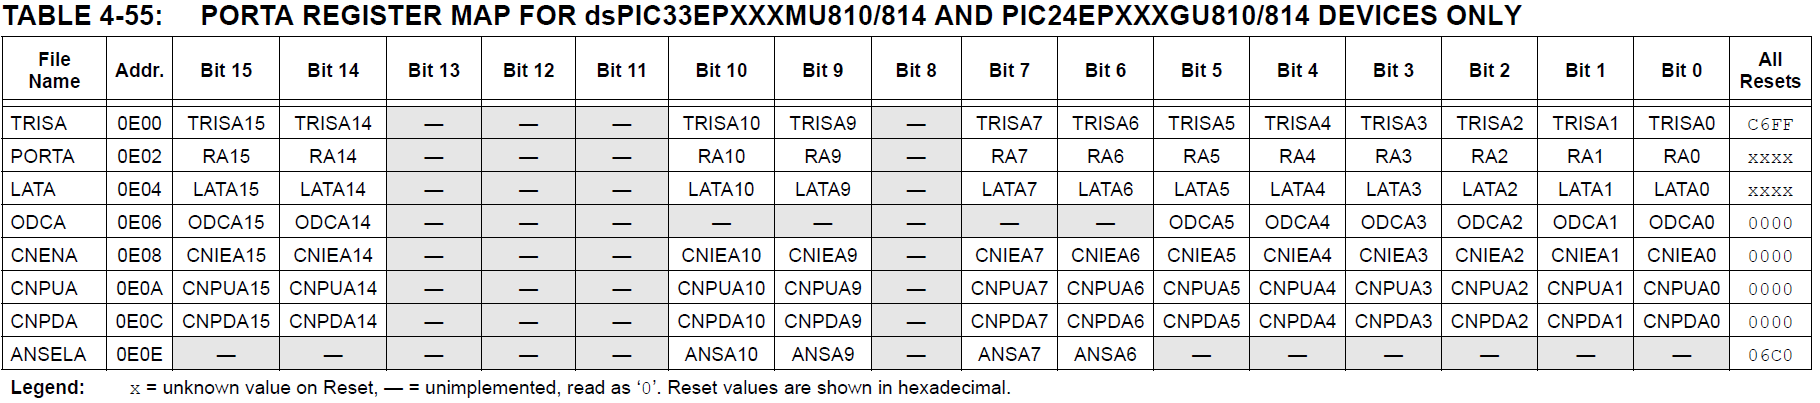
\includegraphics[width=0.8\textwidth]{Images/PORTA}} 
	\subfigure[Register B]{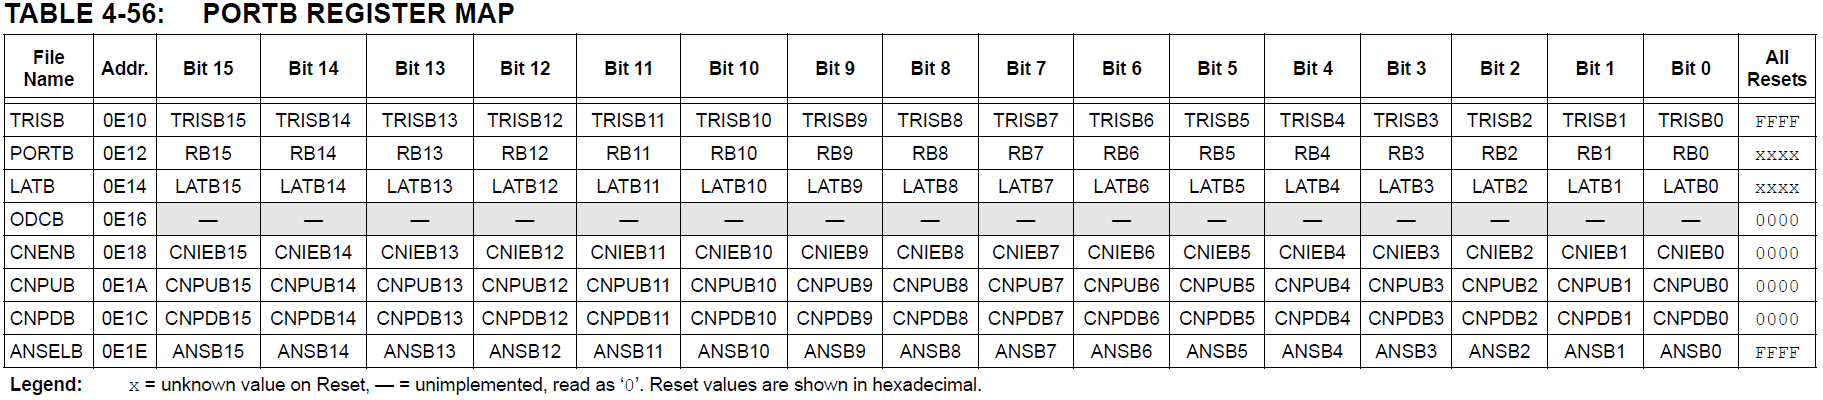
\includegraphics[width=0.8\textwidth]{Images/PORTB}} 
	\subfigure[Register C]{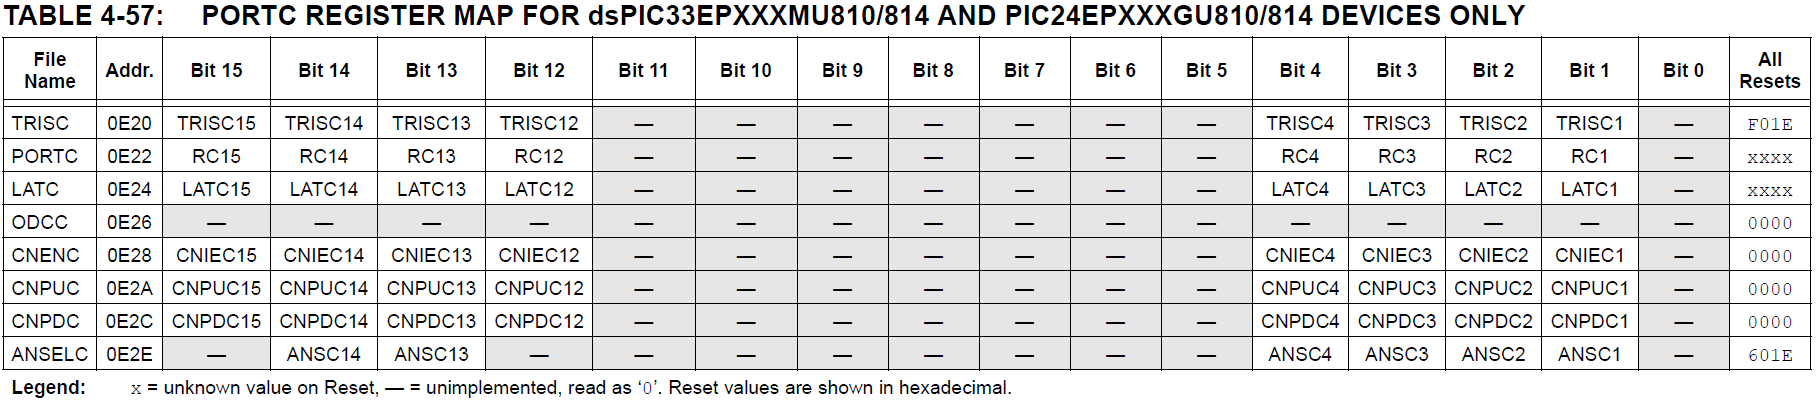
\includegraphics[width=0.8\textwidth]{Images/PORTC}} 
	\subfigure[Register D]{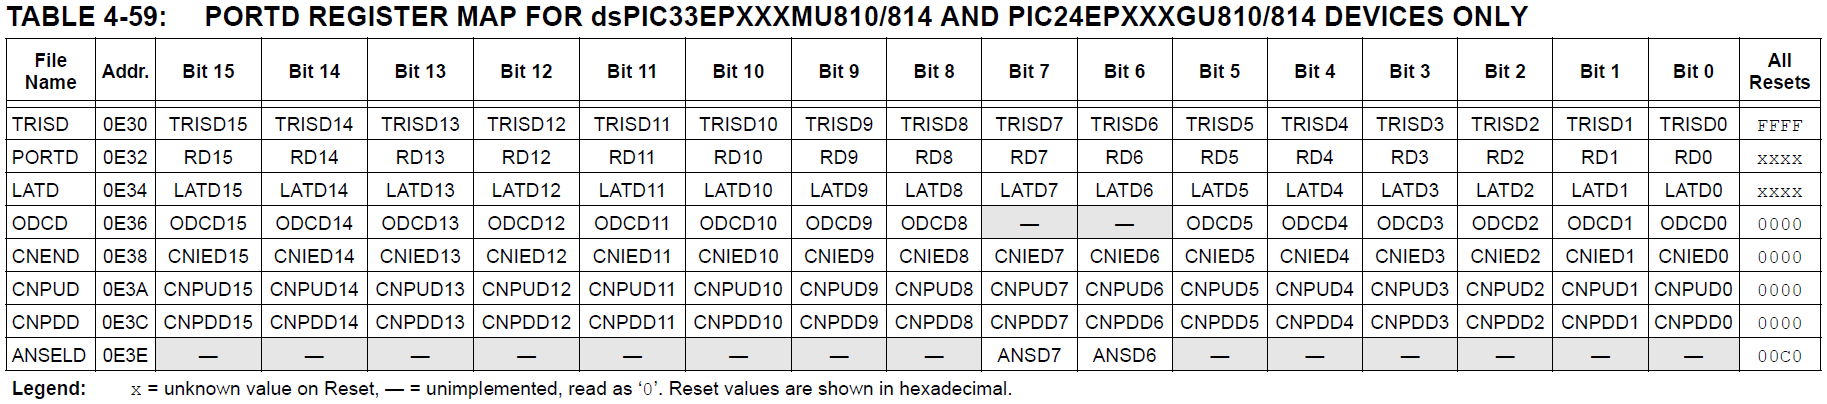
\includegraphics[width=0.8\textwidth]{Images/PORTD}} 
	\subfigure[Register E]{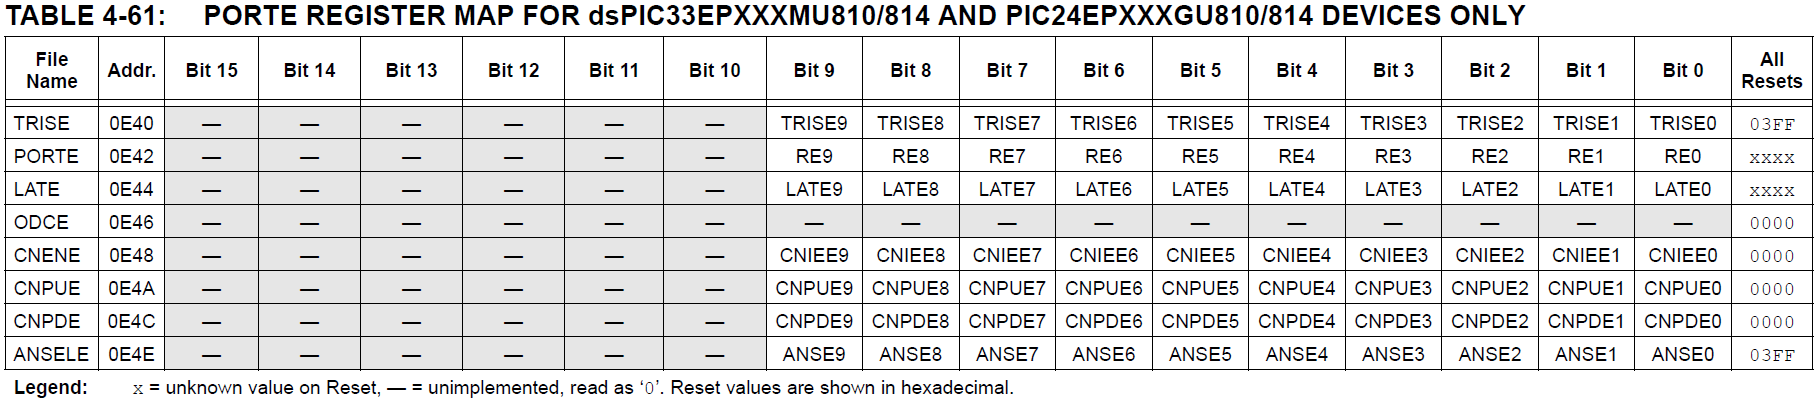
\includegraphics[width=0.8\textwidth]{Images/PORTE}} 
	\subfigure[Register F]{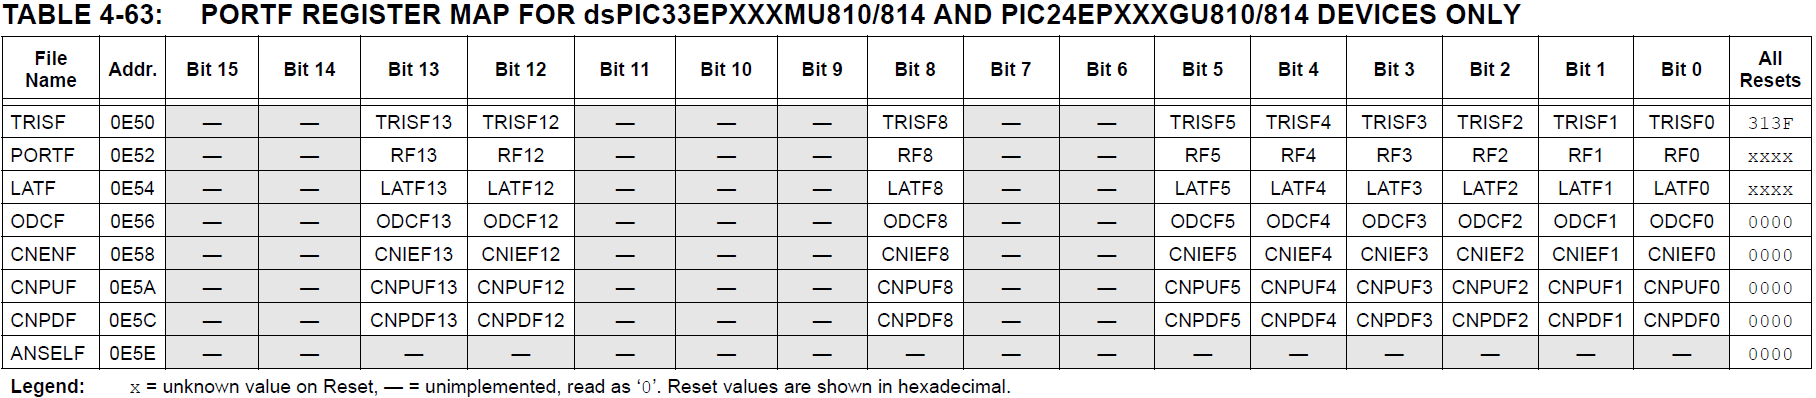
\includegraphics[width=0.8\textwidth]{Images/PORTF}}
	\subfigure[Register G]{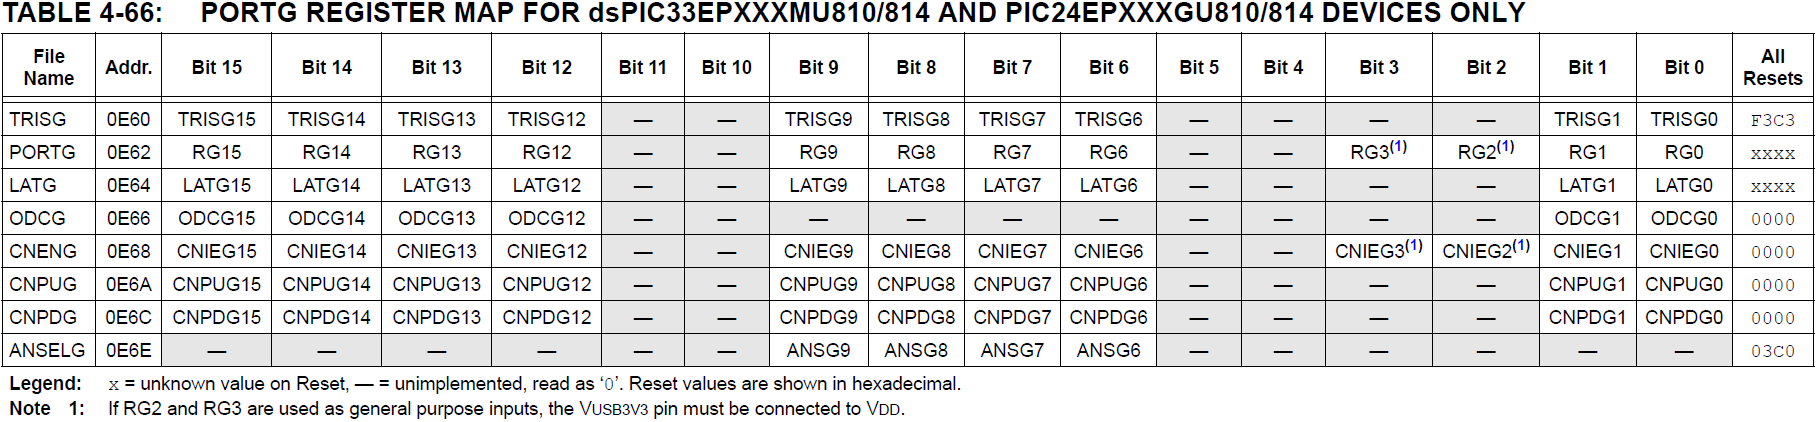
\includegraphics[width=0.8\textwidth]{Images/PORTG}}   
	\caption{PORTA-G Register Map}
	\label{image:PortMap}
\end{figure}

%
%\begin{figure}[h]
%	\centering
%	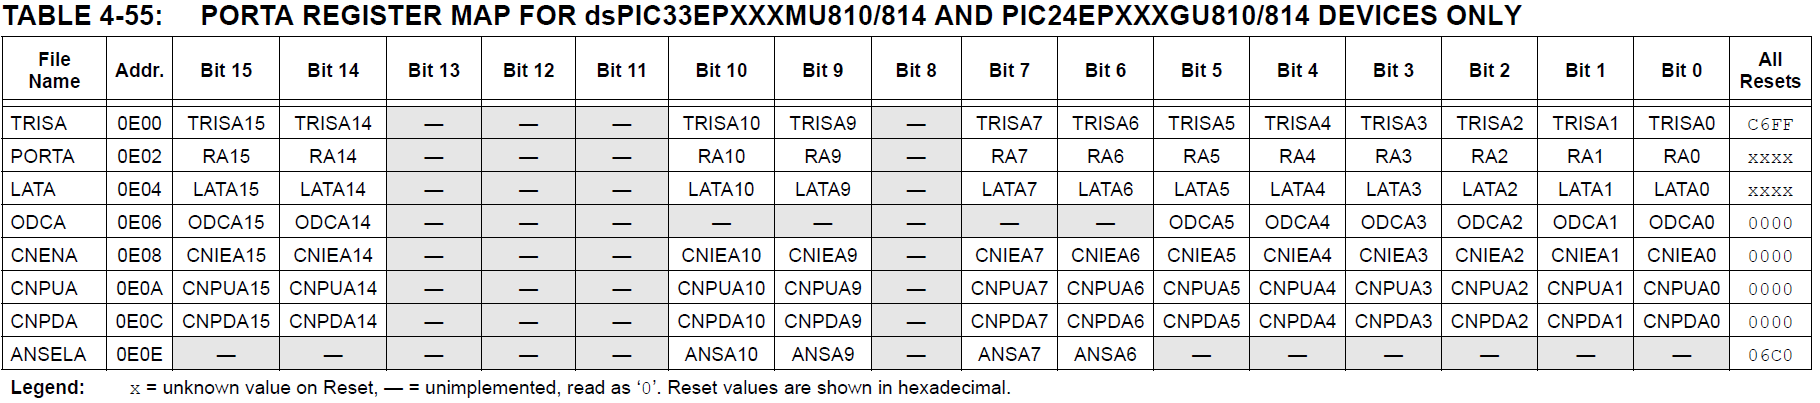
\includegraphics[width=\textwidth]{Images/PORTA}
%	\caption[PORTA Register Map]{PORTA Register Map}
%	\label{image:PORTA}
%\end{figure}
%
%\begin{figure}[h]
%	\centering
%	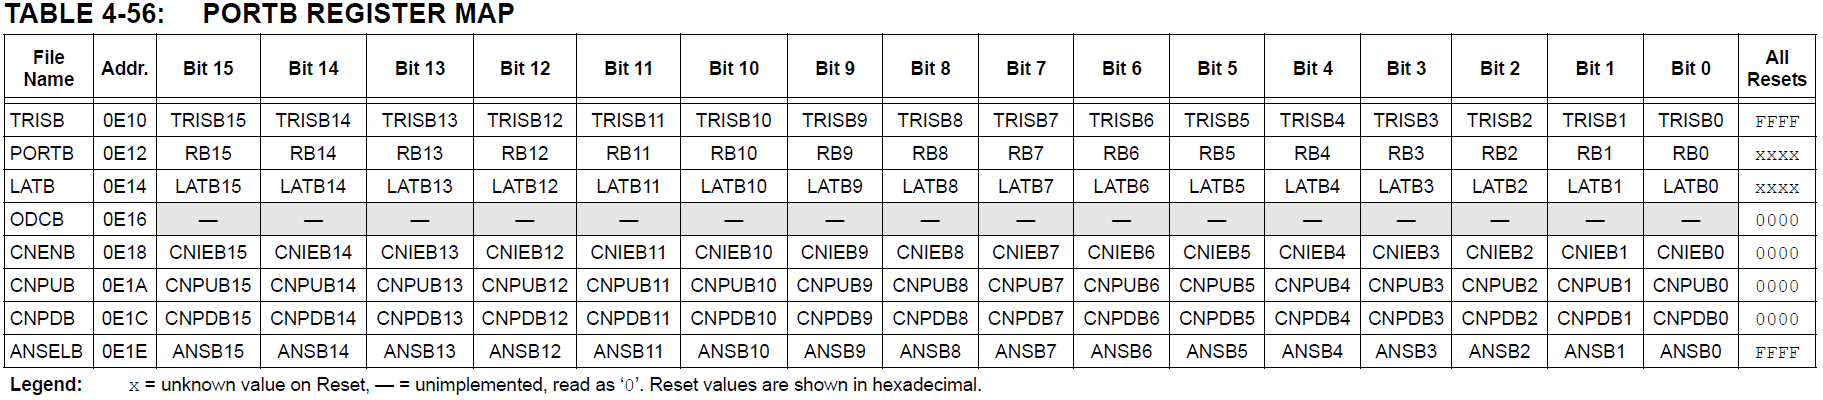
\includegraphics[width=\textwidth]{Images/PORTB}
%	\caption[PORTB Register Map]{PORTB Register Map}
%	\label{image:PORTB}
%\end{figure}
%
%\begin{figure}[h]
%	\centering
%	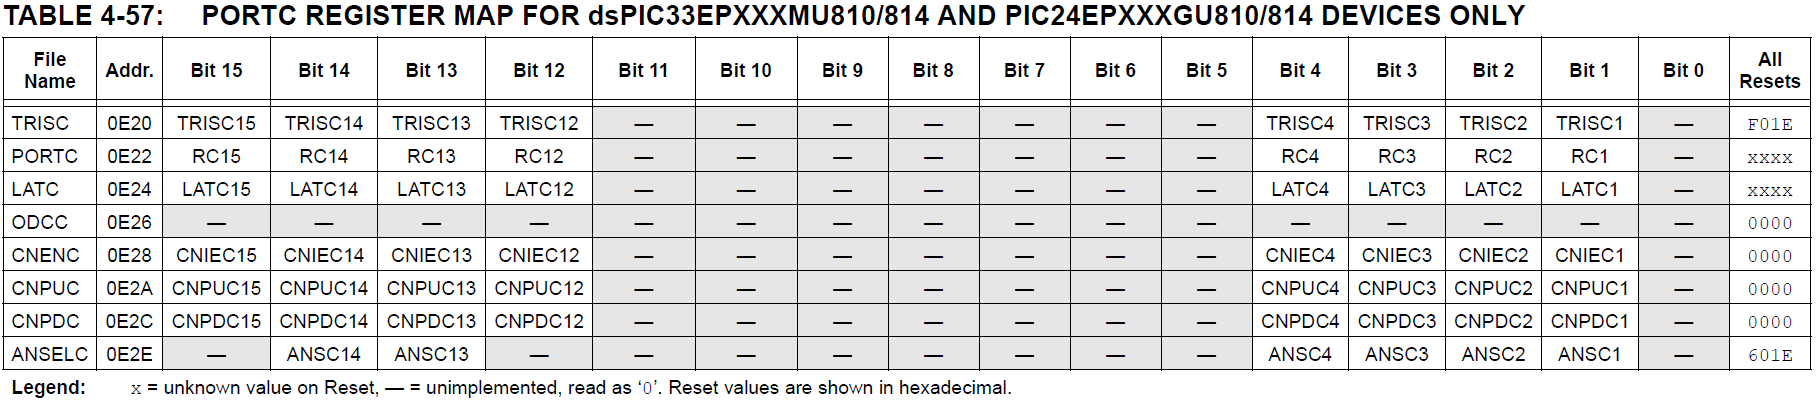
\includegraphics[width=\textwidth]{Images/PORTC}
%	\caption[PORTC Register Map]{PORTC Register Map}
%	\label{image:PORTC}
%\end{figure}
%
%\begin{figure}[h]
%	\centering
%	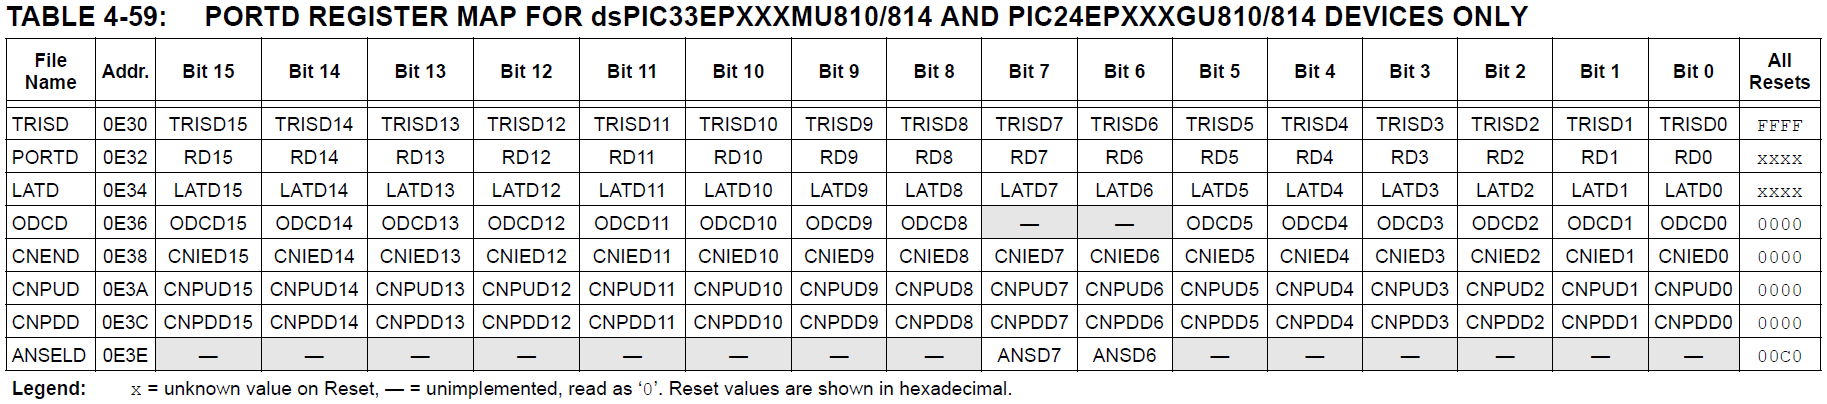
\includegraphics[width=\textwidth]{Images/PORTD}
%	\caption[PORTD Register Map]{PORTD Register Map}
%	\label{image:PORTD}
%\end{figure}
%
%\begin{figure}[!h]
%	\centering
%	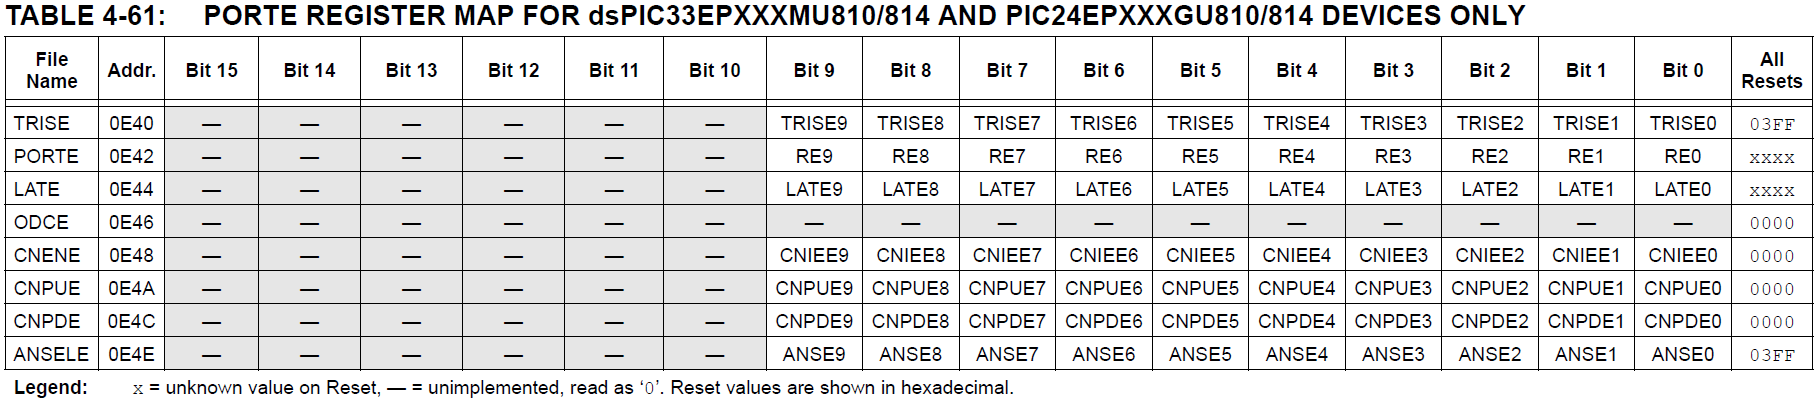
\includegraphics[width=\textwidth]{Images/PORTE}
%	\caption[PORTE Register Map]{PORTE Register Map}
%	\label{image:PORTE}
%\end{figure}
%
%\begin{figure}[!h]
%	\centering
%	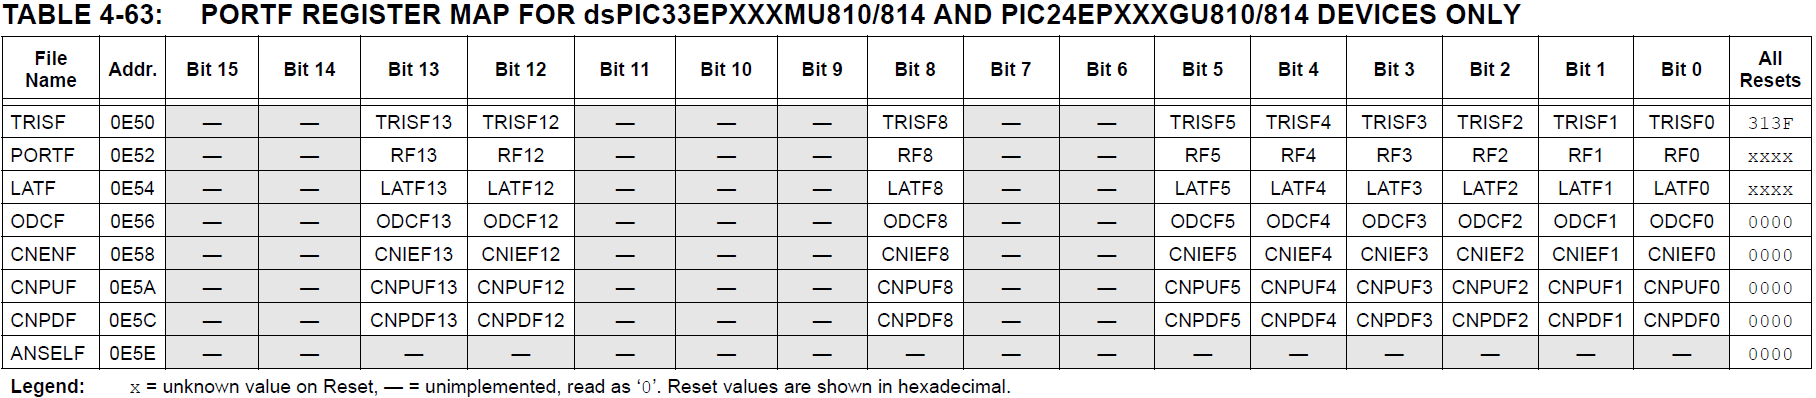
\includegraphics[width=\textwidth]{Images/PORTF}
%	\caption[PORTF Register Map]{PORTF Register Map}
%	\label{image:PORTF}
%\end{figure}
%
%\begin{figure}[!h]
%	\centering
%	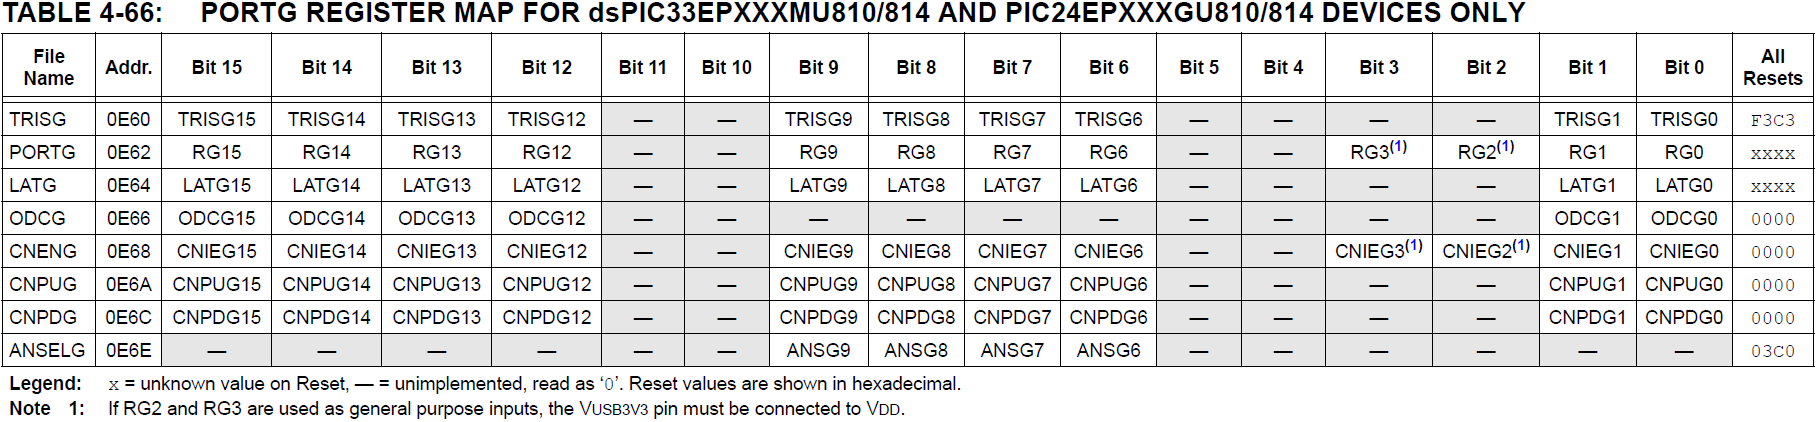
\includegraphics[width=\textwidth]{Images/PORTG}
%	\caption[PORTG Register Map]{PORTG Register Map}
%	\label{image:PORTG}
%\end{figure}

\begin{figure}[!h]
	\centering
	\includegraphics[width=\textwidth]{Images/page207}
	\caption[I/O Ports]{I/O Ports -Datenblatt S.207}
	\label{image:page207}
\end{figure}

\begin{figure}[!h]
	\centering
	\includegraphics[width=\textwidth]{Images/page208}
	\caption[Block Diagramm I/O Ports]{Block Diagramm I/O Ports -Datenblatt S.208}
	\label{image:page208}
\end{figure}	

\begin{figure}[!h]
	\centering
	\includegraphics[width=\textwidth]{Images/page209}
	\caption[I/O Ports]{I/O Ports -Datenblatt S.209}
	\label{image:page209}
\end{figure}

\begin{figure}[!h]
	\centering
	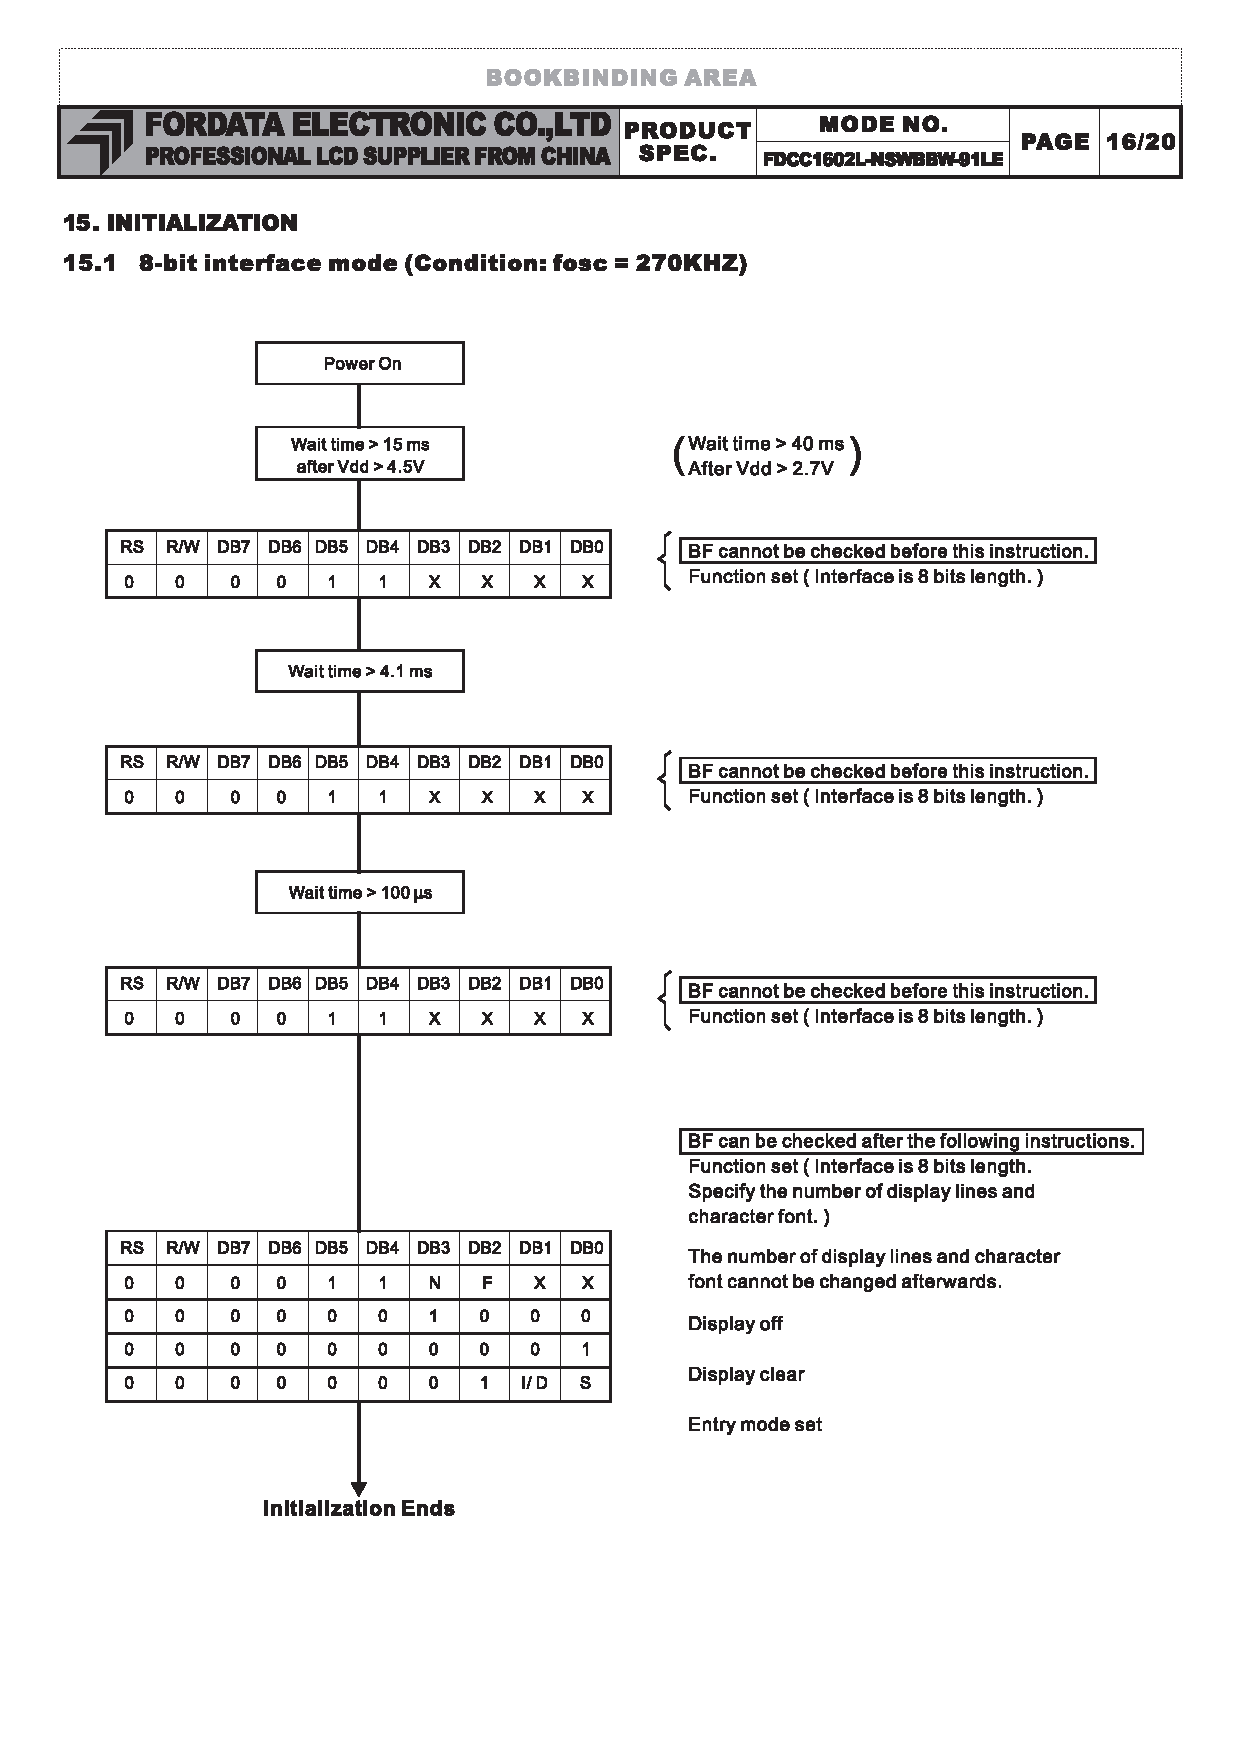
\includegraphics[width=\textwidth]{Images/InitalizationLCD8Bit}
	\caption{LCD Controller Initalization Sequenz}
	\label{image:lcdinit}
\end{figure}


\begin{lstlisting}[frame=htrbl, caption={Initalisierungssequenz des LCD-Controllers}, label={lst:lcdinit}]
void initMyLCD()
{
// 15mS delay after Vdd reaches nnVdc before proceeding with LCD initialization
// not always required and is based on system Vdd rise rate
uint16_t ui16I=0;
while(ui16I++<0xFFFF)Nop();

/* set initial states for the data and control pins */
DATA &= 0xFF00; //set RE0-RE7 low
RW = 0;                         // R/W state set low
RS = 0;                         // RS state set low
E = 0;                          // E state set low

/* set data and control pins to outputs */
TRISE &= 0xFF00;                //set RE0-RE7 to output
RW_TRIS = 0;                    // RW pin set as output
RS_TRIS = 0;                    // RS pin set as output
E_TRIS = 0;                     // E pin set as output

/* 1st LCD initialization sequence */
DATA &= 0xFF00;                 //set RE0-RE7 low
DATA |= 0x0038;                 //set lcd type: 8-bit,2lines,5x7
clockLCDenable();               // toggle E signal
ui16I=0; while(ui16I++<23256)Nop(); //5ms Delay

// 2nd LCD initialization sequence
DATA &= 0xFF00;
DATA |= 0x0038;
clockLCDenable(); 				// toggle Enable signal
ui16I=0; while(ui16I++<4651)Nop(); //200us Delay

// 3rd LCD initialization sequence
DATA &= 0xFF00;
DATA |= 0x0038;
clockLCDenable();
ui16I=0; while(ui16I++<4651)Nop(); //200us Delay

sendCommandLCD( 0x38 );         // function set 8bit, 2lines
sendCommandLCD( 0x0C );         // Display on control, cursor blink off (0x0C), cursor off
sendCommandLCD( 0x06 );         // entry mode set (0x06), increment cursor, no shift 
}
\end{lstlisting}
\newpage

\newpage
\begin{lstlisting}[frame=htrbl, caption={Funktionsprototypen edaPIC33LCD-Library}, label={lst:lcdlib}]
extern char ShadowString[32]; 

void initMyLCD();

void clockLCDenable();

void putcLCD(char c);

void putsLCD(char* pData);

void sendCommandLCD(uint8_t ui8data);

void sendCommandLCDNonBlocking(uint8_t ui8data);

void writeDataLCD(uint8_t ui8data);

void writeDataLCDNonBlocking(uint8_t ui8data);

void setDDRAMAddressLCD(uint8_t ui8address);

uint8_t readBusyFlagLCD();

void putncLCD(char* pData, uint8_t ui8n);

void SendDataToLCD();

void clearLCDStorage();

void SendDataToLCD();

void setLineLCD(const char* pStr, uint8_t ui8Line);

void setLCDLine1(const char* pString);

void setLCDLine2(const char* pString);

\end{lstlisting}
\newpage

\newpage



\end{document}